%%% -*-LaTeX-*-

\chapter{Modulation by very large scales and scale-scale energy transfer to and from large-scale motion}\label{chap:chap2}
The existence of large and very large scale motions (LSMs/VLSMs) in the ABL was reported in previous studies. It was also reported from experimental studies that the large-scale motions modulate the small scales. However, the possible influence of large scales over small scales due to nonlocal turbulent kinetic energy ($tke$) exchange was not examined. Also, the mechanism of spatial development of VLSMs was speculated mostly from visualization of flow features and was not examined in the light of $tke$ exchange. It can be expected that the formation mechanism of LSMs and VLSMs will have some signatures in the energy exchange process between individual scales as governed by the nonlinear term of the Navier-Stokes equations. Here, the modulation effect of large scales on smaller scales is interrogated in the simulated flow fields and the energy exchange between different scales has been explored in the wavelet domain. It has been observed that the energy exchange is not influenced by the presence of VLSMs or different forcing conditions in the examined cases and $tke$ exchange is predominantly local. However, support has been found from the interscale energy exchange process in favour of the hypothesis that LSMs concatenate to give rise to VLSMs.


\section{Introduction}

Many studies have confirmed the existence of Large-Scale and Very Large-Scale Motions (LSMs and VLSMs) throughout the boundary layer in pipe \citep{monty_jfm_07,guala_adrian_jfm2006,baltzer_jfm_13}, channel \citep{monty_jfm_07,balakumar_adrian_ptrs_07,lee_sung_jfm_14,hutchins_marusic_jfm2007,fang2015blm}, and zero pressure gradient boundary layer flows \citep{balakumar_adrian_ptrs_07,Lee_sung_jfm11,hutchins_marusic_jfm2007}. Flow structures corresponding to LSMs and VLSMs can be visually identified in an instantaneous flow field as long streaks of low momentum primarily oriented along the streamwise direction and flanked by similarly shaped high-momentum regions on either side. These structures scale with outer length scales $\delta$, where $\delta$ denotes boundary layer depth, channel half height, pipe radius, etc. depending upon the flow. Monty et al. \citep{monty_jfm_07} measured streamwise velocity with hot wire rakes in a pipe and in a channel and reconstructed the spatial velocity field using Taylor's frozen turbulence hypothesis to visually identify VLSMs. In their study, they observed VLSMs of the order of $25\delta$ in the log layer. Using a similar hot wire apparatus, \citet{hutchins_marusic_jfm2007} also visually identified VLSMs in the log layer of a wind tunnel boundary layer and reported length scales to be found of the order of $20\delta$. They also reported the existence of VLSMs in the buffer layer through their studies of DNS data of channel flow and speculated that correlations likely exist between log-layer-VLSMs and buffer-layer-VLSMs. Using stereoscopic particle image velocimetry data in conjunction with the application of Taylor's frozen turbulence hypothesis, \citet{dennis_nickels_jfm2011} constructed a 3D velocity field from data collected in a water tunnel and showed the 3D structure of VLSMs through a series of iso-surface plots. VLSMs were shown to be low-speed (or high-speed) turbulent bulges inclined with respect to the wall and mainly elongated in the streamwise direction that extend from the wall towards the outer region in the wall-normal direction \citep{dennis_nickels_jfm2011}. Other studies have come to similar conclusions \citep{chung_jfm_10_large,kerherv_roux_etfs_2017}. 

Studies on VLSMs and LSMs are plagued by a lack of an objective definition of these large-scale motions. All visual detection procedures are subjective in nature and a threshold value has to be chosen while visualizing low-momentum or high-momentum regions. \citet{dennis_nickels_jfm2011} appropriately pointed out that choosing a higher threshold may result in underestimation of length of these long structures while inappropriate filtering may smooth away small-scale structures and join smaller structures to give an impression of a single large-scale structure. A more objective definition or detection criteria of the length scales of VLSMs comes from premultiplied 1D spectra of the streamwise velocity component. A bimodal distribution of energy is observed in the premultiplied spectra, where the low wavenumber peak corresponds to VLSMs and the most energy containing relatively large wavenumber mode before a sharp fall-off corresponds to LSMs. This observation of the bimodal distribution has been used to distinguish the two length scales, i.e., LSM and VLSM \citep{kim_adrian_pof99,balakumar_adrian_ptrs_07,guala_adrian_jfm2006}. However, this scale identification from 1D spectra is not devoid of pitfalls. \citet{hutchins_marusic_jfm2007}  pointed out that the meandering nature of the VLSM can cause a shift of the energy peak in premultiplied spectra to shorter wavelengths. Also the approach of extracting a dominant wavelength from energy spectra of the streamwise velocity component to identify VLSMs has an inherent assumption \citep{baltzer_jfm_13} that spatially a low-momentum region would be in immediate vicinity of a high-momentum region of similar length scale in the streamwise direction and, since a VLSM structure represents only a half cycle of a sinusoidal function, the low wavenumber peak in spectra would be indicative of twice the length scale of the VLSM. The issues have been reflected as discrepancies on reported length scales of VLSMs from the premultiplied spectra and visualisation methods. In logarithmic regions of channel and boundary layer flows energy peaks corresponding to wavelengths $7.5\delta$ and $5\delta$ have been reported \citep{balakumar_adrian_ptrs_07}, whereas VLSM length scales of the order of $10\delta$ have been reported from visualizations in both cases \citep{Lee_sung_jfm11,lee_sung_jfm_14,hutchins_marusic_jfm2007}. We feel the need for an alternative approach to asses the importance of VLSMs along with the identification of the probable length scale. 

The wavelet framework offers an alternative approach to look at scale-dependent energy transfers and deduce the important length scales of turbulent dynamics. The most pursued way of analysing scale-to-scale energy transfer involves studying triadic interaction between scales coupled through the nonlinear term in the Fourier domain. Fundamentally, this approach is decoupled from spatial-transport phenomena and the analysis can assess interactions only in a global sense from a spatial point of view due to the nonlocality of sinusoidal functions. The other approach is to study the interaction among scales in both physical space and length scale  space utilising structure functions. In this approach, one attempts to analyze the terms of a diagnostic equation of the turbulent kinetic energy ($tke$) budget derived from the second-order structure function as outlined by Hill \citep{hill_jfm2002}. Marati et al. \citep{marati_jfm_2004} studied an inhomogeneous wall bounded flow using the formulation sketched by Hill \citep{hill_jfm2002}. However, this approach is limited in exploring the length scales bounded by integral-length scales since, structure functions lose physical significance when the auto-correlation drops to a nonsignificant value. 

In this study, we focus on scale-scale energy transfers associated with VLSMs in the atmospheric boundary layer (ABL). The ABL is distinguished from laboratory-scale flows due to the presence of a diurnally varying buoyancy  force and the Coriolis force. Previous studies analyzed length scales of LSMs and VLSMs and the probable mechanisms of their organization, but the question whether weak rotation of the reference frame and atmospheric stability (buoyancy) affects the length scales and organization of these structures remained unanswered. In order to study the effect of Coriolis force on VLSMs, a very large domain of the order of $100\delta$ is desirable given that VLSMs can span a length of $10\delta$. Such requirements poses a fundamental predicament to the DNS approach. Multipoint experimental measurements over such a large domain is also prohibitive, if not impossible. The most practical solution is offered by the large eddy simulation (LES) technique that was used for this study. In order to study two different regimes of large scales and to identify and differentiate their dynamics and significance, a boundary must be delineated between the two regimes of large scales, i.e., LSM and VLSM. We assume that the demarcation scale between LSMs and VLSMs is $\pi\delta$ corresponding to $k_x\delta = 2$ following \citet{guala_adrian_jfm2006}. Since the subjects of this study are VLSMs and LSMs along with the impact of the earth's rotation on them, simulation of very large flow fields was required. To properly resolve length scales as large as $20\delta$,  we chose a domain large enough that these large scales were properly captured as structures advecting freely through the flow field. The possibility that LSMs and VLSMs  interact with smaller scales nonlocally is also explored.  First, we briefly describe the simulation methods and basic flow properties (Sec. \ref{sec:LES_chap2}) and continue with an assessment of the modulating influence of VLSMs on smaller scales as observed from our numerical data set (Sec. \ref{Modulation_VLSMs}).  Section \ref{Analysis of inter-scale energy transfer in wavelet domain} presents the results obtained from analysis of interscale energy transfers in the wavelet domain with a brief introduction to the wavelet method and relevant discussion on LSMs and VLSMs. Finally, we wrap up with a discussion on probable mechanics of developing VLSMs from smaller scale motions. 

\section{Large Eddy Simulations}
\label{sec:LES_chap2}
Three different flow cases were simulated for this study designated as $CHNL$, $EK10$, and $EK02$. $CHNL$ is a classic high Reynold's number channel flow simulation over a large horizontal domain where the flow is sustained by a mean pressure gradient applied across the streamwise ($x$) direction. The mean flow velocity vector in this case points to x-direction. Turbulence is fed off the mean velocity due to instabilities \citep{landahl_christensen_book_92}. The velocity component that contributes most to the turbulent kinetic energy ($tke$) is the x-component of the velocity ($u_1$) and contribution of the spanwise velocity ($u_2$) to the $tke$ is insignificant, unlike in $EK10$ and $EK02$. $EK10$ and $EK02$ are simulations of Ekman layer flows with geostrophic wind velocities ($U_g$) of $10$ m/s and $2$ m/s, respectively (Table \ref{tab:sim_param}). A geostrophic wind condition refers to the balance between the Coriolis force and the mean pressure gradient ($\rho^{-1}\frac{\partial \left < p \right >}{\partial x_i} = f_c\epsilon_{ij3}\tilde{u}_j$) under horizontal homogeneity, and a zero wall-normal stress boundary conditions at the top edge of the BL. Consequently, at the top of the BL, the momentum equation for the z-direction reduces to, $\frac{\partial \left < p \right >}{\partial z} = 0$. In terms of forcing, the key difference between the simulated channel and Ekman cases in this study is that, in $CHNL$, a constant $\left < \rho^{-1} \frac{\partial P}{\partial x} \right >$ sustains the flow while in $EK10$ and $EK02$ a constant $\left < \rho^{-1}\frac{\partial p }{\partial y} \right >  = -f_c U_g$ is acting on the flow, where $f_c$ is the Coriolis parameter. Effectively, the Ekman layer flows are constant pressure gradient flows in a rotating frame of reference. 

All three simulations were carried out in a LES framework where the spatially filtered Navier-Stokes equations for an incompressible flow in the ABL were solved in conjunction with a subgrid-scale stress model. The model equations can be expressed as: 
\begin{align}
    \frac{\partial \tilde{u}_i}{\partial x_{i}} &= 0, \\
    \frac{\partial \tilde{u}_i}{\partial t}+ \frac{\partial \tilde{u}_i\tilde{u}_j}{\partial x_{j}}  &= \frac{-\partial \tilde{p^*}}{\partial x_i}-\frac{\partial \tau_{ij}}{\partial x_j}+ f_{c}\epsilon_{ij3}\tilde{u}_{j},   
\label{eqn:les_eqn}    
\end{align}
\noindent where $i={1,2,3}$ corresponds to $x,y,z$ directions, respectively, ${\tilde{}}$ denotes spatial filtering, $\tilde{u}_i$ denotes the spatially filtered velocity component in the $i$-direction, $\tilde{p^*}=\frac{1}{\rho} \tilde{p}+\frac{1}{3}\tau_{kk}$ is the modified, filtered pressure, the Coriolis parameter has a prescribed value of $10^{-4}$, and $\tau_{ij}$ is the modelled subgrid-scale stress tensor defined as $\tau_{ij}=\widetilde{u_i u_j}-\tilde{u}_i\tilde{u}_j$. $\tau_{ij}$ was modeled with a scale-dependent Lagrangian dynamic subgrid-scale model. Further details of the subgrid-scale model can be found in \citet{stoll_wrr_2006}. The LES code used in this study is pseudo-spectral in nature and uses a Cartesian, staggered grid. Horizontal derivatives are calculated in spectral space while in the surface-normal direction, a second-order-accurate finite-difference approximation is used. Dealiasing was applied through the $3/2$ rule, the lateral boundary conditions were periodic, and the top of the domain utilized a stress free condition, i.e., $\partial\tilde{u}_1/\partial x_3 = \partial \tilde{u}_2/\partial x_3=0$ and the velocity fields were kept divergence free by pressure-correction through the solution of the Poisson equation for the pressure.  All three simulations were run for long enough time to reach a quasi-steady condition. At the wall, instantaneous surface shear stresses, $\tau_{i3,s}(x,y,t)$, were needed as part of the boundary condition, and were computed as a function of the resolved scale velocities $\tilde{u}_1$ and $\tilde{u}_2$ at the lowest vertical nodes at a height of $\Delta_z/2$. This was done using Monin-Obukhov similarity theory as follows:
\begin{align}
\tau_{i3,s}(x,y,t) = -\left [ \frac{\tilde{u}_r(x,y,z,t)\kappa}{\ln(z/z_o)} \right ]^2\frac{\tilde{u}_i(x,y,z,t)}{\tilde{u}_r(x,y,z,t)}, 
\end{align}
\noindent where $\kappa$ is the von K\'arman constant ($=0.4$) and $z_o$ is the local aerodynamic roughness length which was assumed to be $0.1$ m in the simulated cases. The code has been used to simulate the ABL under a variety of different forcing conditions \citep[e.g.,][]{stoll_jas_2009,bailey_blm_2013,miller_blm_2013} and to examine the structure and evolution of turbulent motions \citep[e.g.,][]{bailey_ae_2014,bailey_jfm_2016}.  Its excellent representation of SGS momentum fluxes \citep{stoll_wrr_2006} makes it ideal for an examination of large-scale velocity-field dynamics. In the horizontal directions ($x$, $y$), the extents of the domains ($L_x$, $L_y$) were $128$ Km and in the vertical direction (z), $1.5$, $1.5$, and $0.75$ Km for $CHNL$, $EK10$, and $EK02$, respectively (Table \ref{tab:sim_param}).  To decouple the effect of the Coriolis force from other typical atmospheric conditions such as buoyancy, neutral atmospheric conditions were assumed in all three cases and the effects of rotation were subsequently evaluated. By varying the geostrophic wind velocity, different degrees of rotational effects were observed. 

The filter scales $\Delta_x$ and $\Delta_y$ were the same in the horizontal directions $x$ and $y$, respectively. We took the filtered equations and decomposed the dependent variables further into horizontally  averaged ($\left< \zeta \right>$) and fluctuating components ($\zeta\prime$), where $\zeta$ stands for any of the dependent variables. For convenience, the tilde will be dropped and all dependent variables will be understood as spatially filtered quantities. With the proposed decomposition and under the assumption that this horizontal averaging over statistically independent frames conforms to Reynold's averaging, the transport equation for the turbulent kinetic energy ($q$) takes the following form:
\begin{align}
u_3^\prime u_i^\prime \frac{\partial \left< u_i \right>}{\partial x_3}+[\left< u_j\right>\frac{\partial q}{\partial x_j}+u_j^\prime\frac{\partial q}{\partial x_j}+\frac{\partial }{\partial x_j}(u_i^\prime \tau_{ij}^\prime)]+u_i^\prime\frac{\partial p^\prime}{\partial x_i}+ u_i^\prime \frac{\partial \left < p \right >}{\partial x_i}+u_i^\prime\frac{\partial \left < \tau_{i3} \right >}{\partial x_3}-\tau_{ij}^\prime s_{ij}^\prime =0,
\label{eqn:tke_horz_avg}
\end{align}
\noindent where, $q=\frac{1}{2}u^{\prime}_i u^{\prime}_i$ and $s_{ij}'=\frac{1}{2}(\frac{\partial u_{i}'}{\partial x_j}+\frac{\partial u_{j}'}{\partial x_i})$.
In Equation \ref{eqn:tke_horz_avg}, the first term on the left-hand side denotes production of $tke$ by mean shear, the second term captures the spatial redistribution of $tke$ by the mean flow and turbulence, and the third and fourth terms denote velocity and pressure correlation.  The fifth term stands for redistribution of $tke$ by horizontally averaged subgrid-scale turbulence, and the last term denotes subgrid-scale dissipation by turbulent motions. Although, this equation of $tke$ transport will not be directly analysed in this study, it will serve as a guidepost for the inter-scale energy transfer analysis. In this study a scale dependent version of the combined terms ($-\frac{\partial }{\partial x_i}\left< p^\prime u^\prime\right>-u_j^\prime\frac{\partial \left< q\right>}{\partial x_j}-\frac{\partial}{\partial x_j}\left< u_i^\prime\tau_{ij}^\prime \right>+\left< \tau_{ij}^\prime s_{ij}^\prime\right>$) was analysed via a discrete wavelet framework. Before analysis of the interscale energy exchange, the characteristics of VLSMs are examined to confirm that the same modulating characteristics of VLSMs are observed in simulated flows as was observed in experimental analysis. 

\section{Modulation of Small Scale Fluctuations by VLSMs}
\label{Modulation_VLSMs}

One of the most important identified features of VLSMs is their modulating influence on small scales. Although the precise mechanism of how this modulation takes place has not been definitely identified, through statistical analysis of small-scale fluctuations within an envelope of large-scale fluctuations, the influence can be verified and quantified. \citet{MATHIS2009} conducted tests on the modulating influence of VLSMs on small scales from multipoint measurements in the boundary layer. This was done by isolating the low-frequency envelope of high-frequency (small scale) fluctuations with an application of the Hilbert Transformation and correlating the filtered envelope with the appropriately matched VLSM signal in the near-wall region. A clear signature of long wavelength motions in the log layer modulating smaller scale motions in the roughness sublayer was shown. \citet{Bernardini2011} expanded upon the analysis of \citet{MATHIS2009} and calculated two-point correlations between the small wavenumber envelope of high-wavenumber fluctuations and large-scale fluctuations to demonstrate the appearance of a secondary peak in the amplitude-modulation covariance map. The secondary peak corresponded to long wavelengths and the findings solidified the basic conclusions of \citet{MATHIS2009} and \citet{ganapathi_jfm_2012_modulation}, hereafter referred to as GH12.  GH12 also looked into the amplitude modulation imparted by VLSMs in a high Reynolds number wind tunnel boundary layer utilizing a traversing hot-wire probe. A conditional analysis of small-scale motions as reported in GH12 proved that the amplitude, frequency, and phase of small-scale fluctuations are linked to the same variables of large-scale fluctuations. We adopted the analysis method of GH12 and explored the modulating effect of large-scale motions for the simulation data sets.  Results have been compared with that of GH12 to verify whether LSMs and VLSMs, as detected in the simulation data sets, exhibit similar effects.  For the sake of completeness, a brief description of the analysis is furnished here. For a complete description of the methods, GH12 should be consulted where a descriptive illustration is also presented. The key difference from the analysis of GH12 is that we analyze spatial data whereas, in GH12, the analysis was done on time-series data. To keep the analysis in line with a point measurement of a time series, we treat each streamwise row of the $u_{1}$-component of the velocity and turbulent stress ($u_{1}^{\prime} u_{3}^{\prime}$) as a single data series. Thus, on the $2048 \times 2048$ horizontal grid used here, we get 2048 independent data series at each wall-normal location on the simulation grid.  Four independent instantaneous snapshots of the flow field were taken for each case, thus providing a total of 8192 data sets on each horizontal plane. A brief description of the procedure is summarized below:
\begin{enumerate}[(i)]
\item The fluctuating streamwise velocity component ($u_{1}^\prime(z)$) was separated by subtracting the horizontally averaged velocity ($\left< u_{1}(z)\right>$) from each wall-normal plane from the instantaneous velocity fields.
\item The large-scale component of the fluctuating velocity field ($u_L(z)$) was obtained by filtering $u^\prime(z)$ with a spectral cut-off filter where the cut-off wavelength was $2\delta$ (the red smooth line as shown in Fig. \ref{fig:modulation}). The small-scale fluctuating component was obtained as: $u_s(z)=u^\prime(z)-u_L(z)$ (the cyan dotted line in Fig. \ref{fig:modulation}).
\item In each data, set the series of $u_s(z)$ and $u_L(z)$ were divided into segments of length $2\delta$. Similar segmentation was applied to the turbulent stress ($u_{1}^\prime u_{3}^\prime(z)$) series. Statistics in each individual segment were linked to the representative large-scale fluctuation values. 
\item Large-scale fluctuations were then categorized by a binning process based on the centre value of $u_L(z)$ from each segment of length $2\delta$ as described in step (iii) and as shown with a hypothetical binning in Fig. \ref{fig:modulation}. This process links each individual segment of small-scale data to a $u_L(z)$ bin. In other words, this process gives statistics of small scales conditioned on $u_L(z)$. The number of occurrences of $u_L(z)$ in each bin $N[u_L(z)]$ was counted for all data sets.    
\item In each segment of small scales ($u_s$), the following statistics were calculated:
 \begin{enumerate}[(1)]
    \item The relative variance of the small scales $\Delta u_s^2(u_L,z)$ as: 
    \begin{align}
        \Delta \left < u_s^{2+}\right > =\frac{\left < u_s^2(u_L,z)\right >_S-\left < u_s^2(u_L=0,z)\right >_S}{\left < u_s^2(u_L=0,z)\right >_S} \times 100,
    \label{eq:relative_var_us2}    
    \end{align}
    where $\left < u_s^2(u_L,z) \right >_S = \frac{\sum u_s^2(z)|_{u_L(z)}}{N[u_L(z)]}$ and $\left < u_s^2(u_L=0,z)\right >_S$ denotes $\left < u_s^2(u_L,z) \right >_S$ corresponding to the $u_L=0$ bin.
    \item The average wavenumber of the small-scale fluctuation. This was calculated by counting the number of zero-crossings ($N_m$) and then dividing by 2 ($N_m/2$). Finally, a mean representative wavenumber was calculated as:
    \begin{align}
        \left< k_x|u_L \right> = \frac{\sum k_x(z)}{N[u_L(z)]},
        \label{eq:kx_uL}
    \end{align} 
    where $\sum k_x$ refers to the summation of the average $k_x$ values of all data sets corresponding to an individual $u_L(z)$ bin on a horizontal plane. 
    \item At different surface-parallel planes the mean $\left < u_{1}^\prime u_{3}^\prime\right >$ and variance $\sigma^2_{u_{1}^\prime u_{3}^\prime}$ (of the wall-normal stress ($u_{1}^\prime u_{3}^\prime$)) for each bin were calculated. Finally, a combined mean $\left < u_{1}^\prime u_{3}^\prime \right >_{u_L}$ and a pooled standard deviation ($\sigma^{u_{1}^\prime u_{3}^\prime}_{u_L}$) corresponding to each $u_L$ bin was calculated as: 
    \begin{align}
      \left < u_{1}'u_{3}' \right >_{u_L} = \frac{\sum \left < u_{1}'u_{3}'\right > N_S}{\sum N_S} \ \text{and}
      \label{eq:u'w'_mean}
    \end{align}
    \begin{align}
      \sigma^{u_{1}'u_{3}'}_{u_L} = \sqrt \frac{\sum [\sigma^2_{u_{1}'u_{3}'} + (\left < u_{1}'u_{3}'\right > -\frac{\sum \left < u_{1}'u_{3}'\right >}{\sum N_S})^2 N_S]}{\sum N_S}
     \label{eq:std_uw} 
    \end{align}    
    where the summation ($\sum $) was taken over all segments of the data series on a horizontal plane, corresponding to a single $u_L$ bin. $N_S$ refers to the number of data points in a segment. 
 \end{enumerate}
\end{enumerate}


Figure \ref{fig:us2_uL} shows the strength of small-scale fluctuations conditioned on the magnitude of the fluctuation of large scales, in a relative sense, $ \Delta \left < u_s^{2+}\right >$. The large-scale modulation is measured relative to the weakest large-scale fluctuation corresponding to $u_L=0$, which effectively represents `unmodulated information'. To facilitate the comparison between the three cases, $u_L$ values have been normalized by corresponding friction velocity $u_*$. Any positive change in $ \Delta \left < u_s^{2+}\right >$ should be understood as a percentage amplitude amplification relative to large-scale events corresponding to $u_L/u_*=0$ while a negative change as a percentage attenuation of small-scale intensities compared to a $u_L/u_*=0$ event.  High-momentum large-scale events intensify the small-scale high-velocity events in the surface layer. The higher the momentum-excess in large scales, the higher the strengthening effect on small-scale fluctuations, as is evident from the modulating influence for $u_L/u_*=0.7$ and $u_L/u_*=0.3$ (Fig. \ref{fig:us2_uL}).  Low-momentum large-scale events have the opposite effect on the variance of small-scale fluctuations. Low-velocity large-scale regions  weaken small-scale fluctuation intensities. A low-velocity event of $u_L/u_*=-0.7$ shows more weakening of the small-scale variance than does a $u_L/u_*=-0.3$ event. The effect of high-velocity and low-velocity large-scale events reverses at a height where the surface layer nominally ends. After the crossover point, low-momentum large-scale events intensify the turbulent fluctuations, whereas a high-momentum event at these heights correlates to a turbulence deficit of small scales. The magnitude of modulation by large scales also increases with height beyond the crossover point. The crossover point has been reported to be located at $z^{+}=3.9\sqrt{Re_{\tau}}$ in GH12, where, $z^{+}$ is the wall normal height measured in terms of viscous units and $Re_{\tau}$ is the Reynolds number defined in terms of friction velocity and boundary layer depth $\delta$. In the present study where $Re$ is infinite under the limiting case of inviscid flow the crossover point is observed to be located at $0.18\delta$. The trends of modulation of the small-scale variance by the large-scale fluctuations are similar across the three different flows analyzed. Qualitatively, the results are very similar to those reported in GH12.

The characteristic wavenumber of small-scale motions that are conditioned by the excursions of large scales from the mean flow showed very similar behavior for the three cases (Fig. \ref{fig:kx_ul}).
%Figure \ref{fig:kx_ul} shows the characteristic wavenumber of small-scale motions that are conditioned by the excursions of large scales from the mean flow. 
It is evident from Fig. \ref{fig:kx_ul} that the amplitude of the large-scale motions does not influence the characteristic wavenumber of small scales for a particular case. The general trend of the characteristic wavenumber decreasing in the wall-normal direction indicates that the spatial extent of modulated small scales that are under the influence of large scales increases with height. However, this trend is not monotonous. The modulated small scales grow in spatial extent till nearly 20\% of the boundary layer height and then reache a plateau, finally shifting towards smaller spatial extent again. In general, this agrees with GH12 who observed that the characteristic frequency of small scales decreased with increasing distance from the surface in the region from $y/\delta=0.01-0.6$, after which it plateaued and then increased as the height reached the boundary layer top. In general, a functional independence of the characteristic frequency/wavenumber of small-scale turbulent motions on large-scale fluctuations is manifested in the collapse of lines corresponding to different $u_L$ values. 

A statistical analysis of wall-normal shear stress is also presented in this study to understand the influence of large-scale velocity fluctuations to the turbulent shear stress variations. Figure \ref{fig:uw_uL} shows how excursions of velocity from the mean value in the large scales impact the deviation of turbulent shear stress from the mean along with the range of deviation measured in terms of standard deviations. It is evident that at any wall normal location, the weakest of the large-scale events corresponding to $u_L=0$ causes the highest magnitude of the shear stress. This emphasizes that the mean flow is responsible for majority of the shear stress. The level of fluctuation in the large scales also directly correlates to the magnitude of the shear stress. The higher the magnitude of fluctuation in the large scale, the lower is the contribution to the turbulent shear stress. Also, it is apparent that low-momentum large scale structures tend to contribute more to shear stress than high-momentum structures. The characteristic influence of large-scale structures on shear stress are similar across flow fields analyzed. The effect of modulation of VLSMs on small-scale motions was also studied with a different threshold that separated VLSMs and small-scale motions. The large-scale component of the fluctuating velocity field ($u_L(z)$) was also obtained by filtering $u^\prime(z)$ with a spectral cut-off filter where the cut-off wavelength was $5\delta$. This different threshold value did not impact the observations qualitatively. However, here only results for $2\delta$ cut-off scale are shown.

%================================================ inter-scale energy =========================
\section{Analysis of Interscale Energy Transfer in the Wavelet Domain}
\label{Analysis of inter-scale energy transfer in wavelet domain} 

Before analyzing the energy exchange between individual scales in the wavelet domain, we take a look at the comparison of spectra to discern the turbulent kinetic energy distribution over length scales in different cases.  Premultiplied spectra of the streamwise velocity component averaged over the spanwise direction for all three cases are shown in Fig. \ref{fig:spectra_fw}.  The spectra are normalized with $u_*$ and multiplied by wavenumber $k_{x}$. In the figure, the solid lines represent Fourier spectra, and the circles represent wavelet spectra. In the inertial subrange of turbulence, theory predicts and experimental evidence supports that the velocity spectra will follow a power law resulting in the well-known $-5/3$ spectral scaling (or $-2/3$ for premultiplied spectra) \citep{perry_chng_jfm_86}. The premultiplied spectra for all cases exhibits inertial range scaling with an expected slope of $-2/3$ for normalized wavenumbers $k_xz > 1$. 
%Length scales in the range $k_{x}z < 1$ are expected to show a zero slope in pre-multiplied spectra. 
%These large scales i.e. low wave number modes receive energy from the mean flow and \citet{domaradzki_pof_1994} showed that energy transfer to scales smaller than $0.3\delta$ from the mean flow is negligible in a channel flow characterized by $Re_{\delta}=5000$. 
$CHNL$ has a clear range of scales that fall into zero slope region, while $EK10$ and $EK02$ do not exhibit a range of scale with a matching zero slope. It is apparent in $EK10$ and $EK02$ that normalized wavenumbers of the order of $k_xz=1$ display to have the maximum energy available ,which means that at any height $z$, an eddy of the order of length scale $z$ can be expected to have the maximum energy available. It is also apparent from the figure that at higher heights, the characteristic eddies tend to be shorter than $z$, and at lower heights characteristic eddies tend to be larger than $z$. This indicates the availability of large-scale motions at lower boundary layer. Also a widening of the band of energetic scales with decreasing the wall normal distance is observed. This is consistent with the attached hairpin eddy model of structural organization of a turbulent flow as proposed by \citet{perry_chng_jfm_86, nickels_marusic_jfm_2001} which projects that near the wall more eddies are available to contribute to the energy. The spectra also help to identify dynamically different discrete wavelet scales. For example, it is apparent from Fig. \ref{fig:spectra_fw}(a) and Table \ref{tab:wav-mode2scale} that discrete wavelet scales corresponding to decomposition level $2, 3,\ 4,\ 5, \ \text{and} \ 6$ fall into energy containing scales regime and scales corresponding to level $7,\ 8, \ \text{and} \ 9 $ fall into the inertial subrange regime for the $CHNL$ case. Similarly, all discrete wavelet scales corresponding to different turbulent dynamical regimes can be identified for $EK10$ and $EK02$. Although the spectra reveal the range of important scales in the flow, the dynamics between individual scales cannot be understood. In the following after a brief presentation of the wavelet framework, interscale energy exchange is examined to assess the importance of scale-scale interaction related to VLSMs in the ABL. 

A function in $L^{2}(R^{N})$ can be expanded as a series of orthonormal basis functions and when these orthonormal basis functions consist of scaled and translated versions of a single mother-wavelet function, and a scaling function, the expansion becomes a discrete wavelet expansion. A class of functions that conform to the admissibility condition, are orthogonal to their integer translates, and orthogonal to their own dilations \citep{daubechies88, book_burrus_gopi} are classified as orthogonal wavelets. The discrete scaling ($w_{\phi}(j_o,m,n)$) and wavelet coefficients ($w_{\psi}(j,m,n)$) of a function $\beta(x,y)$ can be obtained from the inner product of the separable basis functions $\phi_{j_o,m,n}$, $\psi_{j,m,n}^{i}$ with the function $\beta(x,y)$ as \citep{dim_gonzalez,book_burrus_gopi,rice_wavelet_toolbox}: 
\begin{align}
& w_{\phi}(j_o,m,n) = \frac{1}{\sqrt{MN}}\sum_{\zeta=0}^{M-1}\sum_{\eta=0}^{N-1}\beta(\zeta\Delta_x,\eta\Delta_y)\phi_{j_o,m,n}(\zeta,\eta) \notag \\ 
& w_{\psi}^q(j,m,n) = \frac{1}{\sqrt{MN}}\sum_{\zeta=0}^{M-1}\sum_{\eta=0}^{N-1}\beta(\zeta\Delta_x,\eta\Delta_y)\psi_{j,m,n}^{i}(\zeta,\eta), \ \ \ q=\{ H,V,D \},
\end{align}
\noindent where $N=M=2^{J}$ are the number of grid points in y and x directions, $\zeta$ and $\eta$ are the grid indices, $\Delta_x$ and $\Delta_y$ are the grid resolutions, respectively in x, y directions and $j_o$ denotes an arbitrary starting scale for the wavelet decomposition, which is unity in this case. The 2D array of scaling coefficients $W_{\phi}(j_o,m,n)$ gives an approximation at scale $j_o$, i.e., low pass filtered version of the analysed function $\beta(x,y)$, while three other 2D zarrays $W_{\psi}^{(H,V,D)}(j,m,n)$ give complementary details to the approximation in horizontal, vertical, and diagonal directions respectively at scales $j \geq j_o$, such that the function $\beta(x,y)$ can be perfectly reconstructed from all the coefficients, where, $j=j_o,j_o+1,j_o+2,...,J-1$; $m,n$ are the number of non-zero filter coefficients of 1D filters that constitute 2D separable wavelet functions. The 2D scaling and wavelet functions are derived from products of 1D functions as follows:
\begin{align}
  \phi(x,y) = \phi(x)\phi(y), \\
  \psi^{H}(x,y)=\phi(x)\psi(y), \\
  \psi^{V}(x,y)=\psi(x)\phi(y), \\
  \psi^{D}(x,y)=\psi(x)\psi(y),
\end{align}
where $\phi(x)$, $\phi(y)$ are one-dimensional scaling, and $\psi(x)$ and $\psi(y)$ are the wavelet functions. The scaled and translated  scaling and wavelet functions at different decomposition levels ($j$) that form the basis of the fast wavelet transform are:
\begin{align}
  \phi_{j,m,n}(x,y)=2^{j/2}\phi(2^{j}x-m, 2^{j}y-n)\ \text{and} \\
  \psi^{i}_{j,m,n}(x,y)=2^{j/2}\psi(2^{j}x-m, 2^{j}y-n), \ \ i=\{H, V, D\}.
\end{align}
The details of implementation of the fast wavelet transform from these functions can be found in \citep{dim_gonzalez,book_burrus_gopi}.

Following \citet{meneveau_91jfm}, any generic dependent variable ($\beta$) obtained from LES can be decomposed into large- and small-scale fluctuations using wavelet filtering,  
\begin{align}
\beta(x,y) = \bar{\beta}(x,y)+\beta(x,y)^{<n} + \beta(x,y)^{>n}
\label{eqn:wavelet_decompos}
\end{align}
where 
\begin{align}
\bar{\beta}(x,y)= \frac{1}{\sqrt{MN}}\sum_m \sum_n w^{}_{\phi}(j_o,m,n)\phi_{j_o,m,n}(x, y),
\end{align}
is the mean horizontal value of $\beta$. $\beta^{<n}$ denotes large-scale fluctuations, which is equivalent to the low-pass filtered portion of $\beta$ where cut-off wavelength is $r_n$, and $\beta^{>n}$ denotes the small-scale counterpart. $\beta^{<n}$ can be obtained from a summation of all wavelet scales larger than the scale represented by $r_n$: 
\begin{align}
 \beta^{<n}(x,y) = \sum_{q=H,V,D} \sum_{j=1}^n  \sum_m \sum_n w^{q}_{\psi}(j,m,n)\psi_{j,m,n}(x, y)\ .
\end{align}
Similarly, the small-scale fluctuating component can be obtained as,  
\begin{align}
 \beta^{>n}(x,y) = \sum_{q=H,V,D} \sum_{j=n+1}^J  \sum_m \sum_n w^{q}_{\psi}(j,m,n)\psi_{j,m,n}(x, y)\ .
\end{align}
In practice, $\beta^{<n}$ is obtained by setting all wavelet coefficients above level $n$ and scaling coefficients to zero and then carrying out the inverse wavelet transform to reconstruct the field from the remaining non-zero coefficients. $\beta^{>n}$ is obtained in a similar fashion by setting all wavelet and scaling coefficients below level $n$ to zero and the inverse wavelet transform from only the scaling coefficients, setting all wavelet coefficients to zero, recovers the mean field ($\bar{\beta}$). $\beta^{>n}$ and $\beta^{<n}$ can be compared to the filtered $\beta$ fields obtained through the application of high-pass and low-pass, spectral-cutoff filters with the cutoff wavenumber $k_{n}$ corresponding to $2\pi/r_n$, respectively. 

 
Expressing velocity and pressure fields as wavelet series, the nonlinear term in the conservation of momentum equation can be decomposed in a manner similar to Leonard's decomposition \citep{leonard1975} with
%\begin{align}
%{\Sigma u_i} \frac{\partial }{\partial t}{\Sigma u_i}+ {\Sigma u_i}\frac{\partial }{\partial x_j}(\Sigma u_i \bar{u}_j+\bar{u}_i\Sigma u_j + \Sigma u_i \Sigma u_j- \left < \Sigma u_i \Sigma u_j\right >) = \Sigma u_i \frac{\partial }{\partial x_i}\Sigma p-\Sigma u_i \frac{\partial }{\partial x_j} \Sigma \tau_{ij},
%\label{tke_wavelet_domain}
%\end{align}
%where, $\Sigma$ indicates summation of all fluctuating scales. Parallels can be drawn between equations (\ref{tke_wavelet_domain}) and (\ref{eqn:tke_horz_avg}). The second term on the left hand side of (\ref{tke_wavelet_domain}) is equivalent to the summation of the convection term of the left hand side and second, and third term on the right hand side of (\ref{eqn:tke_horz_avg}). Summation of the last two terms on the right hand side of (\ref{eqn:tke_horz_avg}) is equivalent to the last term of (\ref{tke_wavelet_domain}) and the pressure correlation terms of these two equations are equivalent. Following Meneveau \cite{meneveau_91jfm} the non linear convection term in (\ref{eqn:les_eqn}) can be broken down into a pseudo cross-stress tensor and Reynolds stress tensor. This results into a pseudo subgrid stress tensor ($T_{ij}$).  
\begin{align} 
u_iu_j = (\bar{u}_i+u_i^{<n}+u_i^{>n})(\bar{u}_j+u_j^{<n}+u_j^{>n})\ , 
\end{align}
which can be rearranged to define a term $T_{ij}$ that represents the summation of the pseudo cross-stress tensor  that accounts for interactions among large- and small-scale turbulent motions and the Reynold's stress tensor as:  
\begin{align}
u_iu_j-\Gamma-u_i^{<n}u_j^{<n} & = u_i^{>n}u_j^{<n} + u_i^{<n}u_j^{>n} + u_i^{>n}u_j^{>n}= \theta_{ij} , 
\label{wavelet_pseudo_stress}
\end{align}
where, $\Gamma   = \bar{u}_i\bar{u}_j+u_i^{<n}\bar{u}_j+u_i^{>n}\bar{u}_j+\bar{u}_iu_j^{<n}+\bar{u}_iu_j^{>n}$ and $u_{i}^{<n}u_{j}^{<n}$ is the Reynold's stress for fluctuations below decomposition level $n$.
%\[ \mathbf{I}=  \frac{1}{\sqrt{MN}}\sum_{q=H,V,D}  \sum_{m}\sum_{n}\psi_{j,m,n}\partial_{j}[\psi_{j,m,n}\psi_{j,m,n} + \psi_{j,m,n}\phi_{j_{o},m.n}] \]

%The subgrid stress tensor ($\tau_{ij}$) as obtained from the LES can also be broken down into a large and small scales.
%\begin{align}
%  \tau_{ij} = \tau_{ij}^{<n}+\tau_{ij}^{>n}
%  \label{eqn:tau_breakdown}
%\end{align}
%Inherent into this decomposition of the SGS stress tensor is the assumption that Smagorinsky coefficient i.e. eddy viscosity is scale independent although, in the LES scale dependent Smagorinsky model with Lagrangian averaging was used. Using the decomposition in (\ref{wavelet_pseudo_stress}). 
For convenience, we have adopted the Meneveau's notation and will denote wavelet coefficient of the velocity fields at scale $m$ as $ w^{m,q}_{\psi}[\mathbf{i}]$ and that of all other variables as $[\ ]^{(m,q)}_{\psi}[\mathbf{i}]$. The transport equation of $tke$ for the scale $r_m$ can be written as: 
\begin{align}
& \frac{\partial}{\partial t}(w_{\psi}^{(m,q)})^2[\mathbf{i}]+ w_{\psi}^{(m,q)}[\mathbf{i}] \left [ \frac{\partial }{\partial x_{j}}(u_i^{<n}u_j^{<n}+\Gamma) \right ]_{\psi}^{(m,q)}[\mathbf{i}]   =  \nonumber \\ & -w_{\psi}^{(m,q)}[\mathbf{i}] \left [ \frac{\partial}{\partial x_i}(p^{<n}) \right ]_{\psi}^{(m,q)} [\mathbf{i}]-w_{\psi}^{(m,q)}[\mathbf{i}] \left [ \frac{\partial p^{>n}}{\partial x_i}+\frac{\partial}{\partial x_j}( \theta_{ij}+\tau_{ij} ) \right ]_{\psi}^{(m,q)}[\mathbf{i}],     
\label{eqn:tke_eqn_m_level}
\end{align} 
where the last term in Eqn. \ref{eqn:tke_eqn_m_level} encompasses the nonlinear interactions across scales and here is used to define   
\begin{align}
  t^{(m,n)}= \sum_{i=1}^2\sum_{q=1}^{3}w_{\psi}^{(m,q)}[\mathbf{i}] \left [ \frac{\partial p^{>n}}{\partial x_i} +\frac{\partial}{\partial x_j}\left ( \theta_{ij}+\tau_{ij}\right )\right ]_{\psi}^{(m,q)}[\mathbf{i}].
\end{align} 
The term $t^{(m,n)}$ that accounts for the transfer of energy between scales $r_m$ and all scales smaller then $r_n$ ($r_m \geq r_n$) can be recovered from the decomposition in \ref{wavelet_pseudo_stress}. \citet{{meneveau_91jfm}} explained the term $t^{(m,n)}$ as an alternative to the scale-scale transfer term $G(k|k_n)$ representing the nonlinear interactions among turbulent scales in the Fourier domain such that $G(k|k_n)$ demotes the aggregate effect of nonlinear interactions to wavenumber $k$ due to interactions among triads of scales $(k,\ p,\ k-p)$ where, ``$k < k_n$ and at least one of the other two legs is larger than $k_n$". A similitude of $t^{(m,n)}$ can be drawn with  the detailed triadic interactions as formulated in the spectral space by \citet{domaradzki_pof_1994}: 
\begin{align}
t^{(m,n)} \approx \sum_{p=1}^{k_{max}} \sum_{q>k_n}^{k_{max}} G^{pqm}.
\end{align}
A negative value of $t^{(m,n)}$ represents energy loss from the scale $r_m$ and a positive value indicates energy transfer to scale $r_m$ from scales smaller than $r_n$, i.e., backscatter. The same filter scale ($r_m/r_n$) must be used in both horizontal directions and thus, a single ($m/n$) integer is used to represent the filter scale. This is in contrast to spectral space where a wide array of wave vectors that obey the triangle relation $\bar{\mathbf{p}}+\bar{\mathbf{q}}=\bar{\mathbf{m}}$ can interact nonlinearly. The disadvantage is that while spectral space allows one to probe into the detailed triadic scale interactions, a local-spatial distribution of energy cannot be obtained. Wavelet space in spite of limitations of entangling spatial transport with scale-scale interaction provides an opportunity to explore spatial distribution of scale-scale interactions that can be used to develop an understanding of the sparsity of turbulent energy and quantify its intermittency \citep{dunn_jfm_2003, dunn_cf2005,meneveau_91jfm}. 

A dual bi-spectrum of subgrid energy exchange can be defined from $t^{(m,n)}$ following \citet{{meneveau_91jfm}} as, 
\begin{align}
  T(z,k_m|k_n) = \frac{2^{-(J-n)}(\Delta x \Delta y)^{1/2}t^{(m,n)} }{2\pi\ln(2)}. 
\end{align}
Figures \ref{fig:tmn_fixed_n_chnl}, \ref{fig:tmn_fixed_n_ek10}, \ref{fig:tmn_fixed_n_ek02} and \ref{fig:tmn_fixed_n_meqn_chnl}, \ref{fig:tmn_fixed_n_meqn_ek10}, \ref{fig:tmn_fixed_n_meqn_ek02} show the dual bi-spectrum of subgrid scale energy spectra, i.e., the rate of energy transfer per unit area per unit length of scale, $T(z,k_m|k_n)$, at different horizontal planes above the ground. The results shown in Fig. \ref{fig:tmn_fixed_n_chnl}, \ref{fig:tmn_fixed_n_ek10}, \ref{fig:tmn_fixed_n_ek02} and \ref{fig:tmn_fixed_n_meqn_chnl}, \ref{fig:tmn_fixed_n_meqn_ek10}, \ref{fig:tmn_fixed_n_meqn_ek02} differ in their definition of $T(z,k_m|k_n)$. Fig. \ref{fig:tmn_fixed_n_chnl}, \ref{fig:tmn_fixed_n_ek10}, \ref{fig:tmn_fixed_n_ek02} use a definition of $T(z,k_m|k_n)$ where the filter scale $r_n$ is always  smaller than $r_m$ and interaction among triads of scales are considered where at least one of the scale is $\leq \frac{1}{2}r_m$. In Fig. \ref{fig:tmn_fixed_n_meqn_chnl}, \ref{fig:tmn_fixed_n_meqn_ek10}, \ref{fig:tmn_fixed_n_meqn_ek02}, $T(z,k_m|k_n)$ is due to interactions of scales $r_m$ with scale $r_m$ and scales smaller than $r_m$. In Fig. \ref{fig:tmn_fixed_n_chnl}, \ref{fig:tmn_fixed_n_ek10}, \ref{fig:tmn_fixed_n_ek02} backscattering events far outnumber forward energy cascade events. However, a comparison between Fig. \ref{fig:tmn_fixed_n_chnl}, \ref{fig:tmn_fixed_n_ek10}, \ref{fig:tmn_fixed_n_ek02} and \ref{fig:tmn_fixed_n_meqn_chnl}, \ref{fig:tmn_fixed_n_meqn_ek10}, \ref{fig:tmn_fixed_n_meqn_ek02} shows that for any particular scale, energy exchange due to interactions between neighbouring scales dwarfs interactions between distant scales. In Fig. \ref{fig:tmn_fixed_n_meqn_chnl}, \ref{fig:tmn_fixed_n_meqn_ek10}, \ref{fig:tmn_fixed_n_meqn_ek02} forward cascade of energy is dominant over backscattering. In most of the cases, it is the neighbouring scale in terms of dyadic wavelet scales where most of the energy exchange for any fixed $r_n$ occurs irrespective of the direction of energy transfer. 

Although the discrete wavelet transform is limited only to dyadic scales, local and nonlocal energy transfer can be identified in the limiting cases. Studies that looked into turbulent energy exchange between scales in the Fourier space defined local versus non-local energy transfers in relation to the smallest and the largest scale in the triad. If $k,p, \text{and}\ q$ are the three wavemodes of the nonlinear term obeying the condition $k+p+q=0$, the ratio between the maximum and the minimum length scales can be defined as $s=max(k,p,q)/min(k,p,q)$. \citet{domaradzki_pof_1994} and \citet{bourouiba_straub_jfm11} categorized interaction between scales as a local if $s\leq 2$ and nonlocal if $s\geq 2$. Under this definition of locality of scales, it can be concluded that energy transfer is predominantly local for all scales larger or of the order of LSMs in all cases. This trend is observed throughout the boundary layer. Two instances of nonlocal energy transfer are observed in $CHNL$ (Fig. \ref{fig:tmn_fixed_n_chnl}). All scales smaller than $0.08\delta$ are observed to be receiving a relatively higher amount of energy from distant scales $0.33\delta$ and $0.67\delta$. A similar nonlinear interaction is observed when scales smaller than $0.17\delta$ interact with scale $0.67\delta$. Also, energy contribution to scales smaller than $0.17\delta$ from $0.33\delta$ and $0.67\delta$ are comparable. In  $Ek10$, one instance of nonlocal interaction is observed within the analyzed range of scales. Scale $0.35\delta$ tend to contribute more subgrid energy to scales smaller than $0.09\delta$ as compared to scale $0.17\delta$ (Fig. \ref{fig:tmn_fixed_n_ek10}). $EK02$ shows mostly local interaction among scales within the analyzed range (Fig. \ref{fig:tmn_fixed_n_ek02}). All the observed nonlocal interactions are attributed to scales smaller than or at the lower end of the presumed definition of LSMs. It can for this reason be concluded that VLSMs do not influence the dynamics of smaller scale motions through nonlocal interactions while LSMs have the potential to have nonlocal impact for some range of scales. It must be emphasized that the relative contribution of nonlocal transfers in backscattering is very small compared to local transfer (Fig. \ref{fig:tmn_fixed_n_meqn_chnl}, \ref{fig:tmn_fixed_n_meqn_ek10}, \ref{fig:tmn_fixed_n_meqn_ek02}). In Fig. \ref{fig:tmn_fixed_n_meqn_chnl}, \ref{fig:tmn_fixed_n_meqn_ek10}, \ref{fig:tmn_fixed_n_meqn_ek02}, backscattering is observed only above the log region in all three cases. Scale-scale interaction show differences in $EK02$ compared to $EK10$ and $CHNL$ including markedly less of a tendency of backscattering. 

From the definition of $t^{(m,n)}$ a local subgrid-scale flux of energy can be calculated by summing $t^{(m,n)}$ over $m$, 
\begin{align}
\Pi_{sg}^{n}(z)[\mathbf{i}] = -\sum_{m=1}^{n}2^{2n}t^{(m,n)}[2^{(m-n)}\mathbf{i}],
\label{pi_tmn}
\end{align}
\noindent where $\Pi_{sg}^{n}$ quantifies the summation of energy transfer from all scales larger or equal to $r_m$ to scales smaller than $r_n$. According to the current definition, a positive value of $\Pi_{sg}^{n}$ would refer to energy transfer from large to small scales and a negative value would indicate energy transfer from small to large scales, i.e., backscatter. From $\Pi_{sg}^{n}$, a subgrid energy flux spectra is defined as: $\pi_{sg}^{n}= 2^{-2(M-n)}\left < \Pi_{sg}^{n} \right >$, which quantifies rate of local energy dissipation per unit area from scales larger than $r_n$.  \citet{meneveau_91jfm} explained this term as a surrogate of the LES term that quantifies energy transfer between resolved and sub-grid scale motions, i.e., ($\tilde{u}_i\frac{\partial }{\partial x_j}(\widetilde{u_iu_j}-\widetilde{\tilde{u}_i\tilde{u_j}})$). In case of a homogeneous flow, this analogy is straightforward; however, for any wall bounded flow where heterogeneity is strong at least in one direction, this should be understood with caution and for variables filtered appropriately in the homogeneous directions only. In this study, where homogeneity can only be assumed in horizontal directions $\pi^{n}_{sg}$ calculated in a wavelet filtering framework is analogous to ($\tilde{u}_i\frac{\partial }{\partial x_j}(\widetilde{u_iu_j}-\widetilde{\tilde{u}_i\tilde{u_j}})$), where variables are filtered with a 2D filter on surface-parallel planes. The turbulent flow field at any wall-normal location ($z$) was obtained by subtracting convection velocity $\left < u \right >(z)$, where $\left < u \right > (z)$ was the mean horizontal velocity assumed steady after the simulation had reached a quasi-steady condition. In practice, these assumptions allowed us to treat the velocity field represented by wavelet scaling coefficients as one for which inverse wavelet transform  would yield the average velocity field with a convection velocity of $\left < u \right > (z)$. $\pi^{n}_{sg}$  can also be understood as a scale-dependent version of the combined terms ($-\frac{\partial }{\partial x_i}\left < p'u'\right>-u_j'\frac{\partial \left < q\right >}{\partial x_j}-\frac{\partial }{\partial x_j}\left < u_i'\tau_{ij}'\right >+\left < \tau_{ij}'s_{ij}'\right >$) in Eqn. \ref{eqn:tke_horz_avg}. In Fig. \ref{fig:pi_tmn}, horizontally averaged scale-dependent subgrid-scale energy transfer $\left < \pi^{n}_{sg} \right >$ is shown. Panels $a^\prime$, $b^\prime$, and $c^\prime$ on the right-hand side of Fig. \ref{fig:pi_tmn} show the results corresponding to Eqn. \ref{pi_tmn}. Panels $a$, $b$, and $c$ on the left shows $\left < \pi_{sg}^{\prime n} \right >$.  Subgrid energy flux spectra $\left < \pi_{sg}^{\prime n} \right >$ differs from $\left < \pi_{sg}^{n} \right >$ as defined in Eqn. \ref{pi_tmn}. $\left < \pi_{sg}^{\prime n} \right >$ is derived from  a slightly different definition of $\Pi_{sg}^{n}$ than Eq. \ref{pi_tmn} as follows: 
\begin{align}
\Pi_{sg}^{\prime n}(z)[\mathbf{i}] = -\sum_{m=1}^{n-1}2^{2n}t^{(m,n)}[2^{(m-n)}\mathbf{i}].
\label{pi_tmn_1}
\end{align}
The difference between $\pi^{n}_{sg}$ and $\pi^{\prime n}_{sg}$ is that the former term accounts for the energy transfer occurring between scales of spatial extent of $r_n$, and all scales equal to $r_n$ or smaller, while the later only includes aggregate results of interaction between all scales larger than $r_m$ and smaller than $r_n$.  Substantial difference between $\pi^{n}_{sg}$ and $\pi^{\prime n}_{sg}$ suggests that within the interrogated wavelet scale regime where integer length scales are distributed over $log(2)$ scale, interactions among the similar spatial scales dominate the subgrid-scale energy transfer. In Fig. \ref{fig:pi_tmn}, $\pi^{n}_{sg}$ and $\pi^{\prime n}_{sg}$ are normalized by estimated dissipation in the log layer. Using the relevant velocity scale ($u_*$) in the internal ABL and an estimated velocity gradient in the log layer derived from similarity theory, an energy scale relevant in the log layer can be formed as $u^3_*/(\Delta z \kappa)$, where $\Delta z$ is the resolution of the simulation in the wall normal direction, i.e., distance of the first u-node in wall normal direction \citep{book-garrat-blm}. This energy estimate is the expected order of energy to exist in the surface layer. Panels $a$, $b$, and $c$ in Fig. \ref{fig:pi_tmn} indicate that local subgrid-scale energy transfer due to interactions of distant scales on an average is negative, i.e., backscatter. This trend is consistent across all three cases and throughout the boundary layer. Smaller scales are observed to transfer higher amounts of energy to larger scales. For example, in Fig. \ref{fig:pi_tmn}(a), all scales smaller than $r_n=0.08\delta$ are observed to transfer more energy to scales larger than $0.17\delta$ compared to the total energy transfer from scales smaller than $0.17\delta$ to scales larger than $0.33\delta$. Panels $a'$, $b'$, and $c'$ show plane average $\pi^{\prime \ n}_{sg}$ and show a very different distribution  compared to plane average $\pi^{n}_{sg}$. The quantity $\pi^{\prime n}_{sg}$ accounts for the interaction of similar length scales. However, the spatial transport $\left \{ \frac{\partial }{\partial x_j}(u_i\tau_{ij})\right \}$ due to interaction of large scales with a band of small scales cannot be separated in this formulation while analysing the energy transfer $\left ( \tau_{ij}S_{ij} \right )$  due to lack of a simple relation between wavelets and its derivatives as was pointed out by \citet{meneveau_91jfm}.

%\graphicspath{{chap2Img/}}
%\begin{figure}[htb]
%\centering {
%	\begin{minipage}{0.333\textwidth}
%	  \begin{picture}(100,150)
%		  \put(0,0){{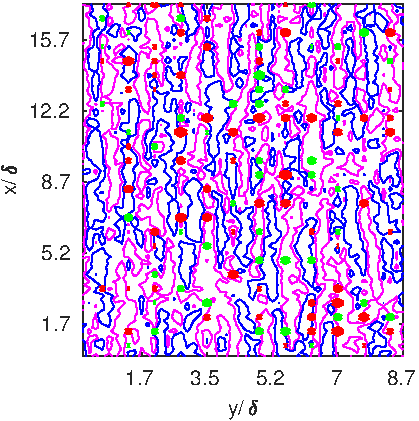
\includegraphics[width=2in,height=2in]{ek10_pi_2d_n_9_m_9_lvl_33-eps-converted-to}}}{}% 
%		  \put(0,150){(a)}
%		\end{picture}
%	\end{minipage}%
%	\begin{minipage}{0.333\textwidth}
%	    \begin{picture}(100,150)
%		    \put(0,0){{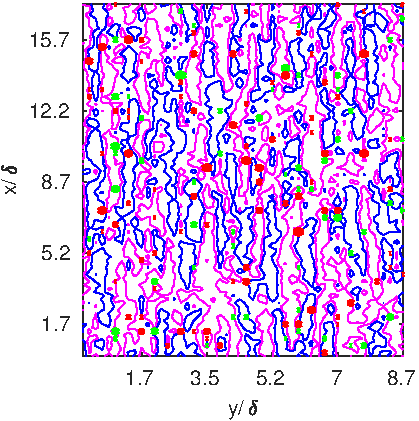
\includegraphics[width=2in,height=2in]{ek10_pi_2d_n_9_m_8_lvl_33-eps-converted-to}}}{}% 
%		    \put(0,150){(b)}
%		  \end{picture}
%	\end{minipage}%	
%	\begin{minipage}{0.334\textwidth}
%	  \begin{picture}(100,150)
%		  \put(0,0){{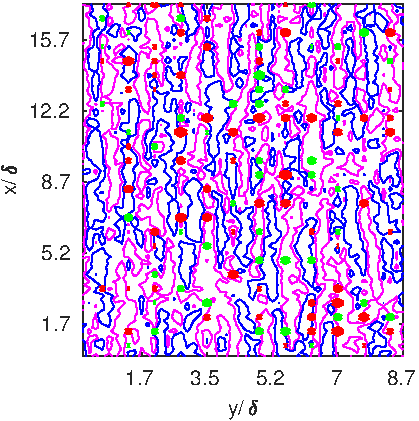
\includegraphics[width=2in,height=2in]{ek10_pi_2d_n_9_m_7_lvl_33-eps-converted-to}}}{}% 
%		  \put(0,150){(c)}
%		\end{picture}
%  \end{minipage}	
%  
%	\begin{minipage}{0.333\textwidth}
%	  \begin{picture}(100,150)
%		  \put(0,0){{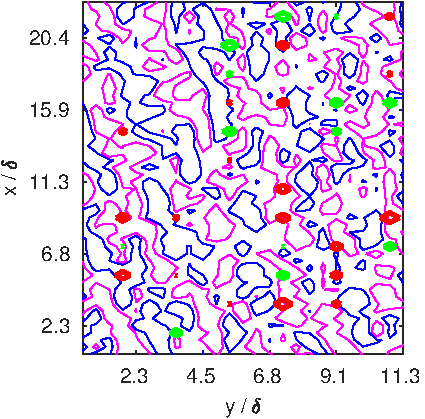
\includegraphics[width=2in,height=2in]{ek02_pi_2d_n_9_m_9_lvl_25-eps-converted-to}}}{}% 
%		  \put(0,150){(d)}
%		\end{picture}
%	\end{minipage}%
%	\begin{minipage}{0.333\textwidth}
%	    \begin{picture}(100,150)
%		    \put(0,0){{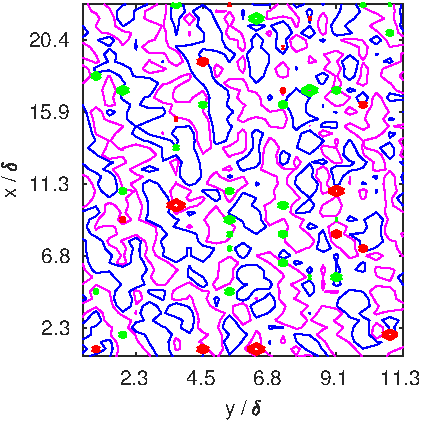
\includegraphics[width=2in,height=2in]{ek02_pi_2d_n_9_m_8_lvl_25-eps-converted-to}}}{}% 
%		    \put(0,150){(e)}
%		  \end{picture}
%	\end{minipage}%	
%	\begin{minipage}{0.334\textwidth}
%	  \begin{picture}(100,150)
%		  \put(0,0){{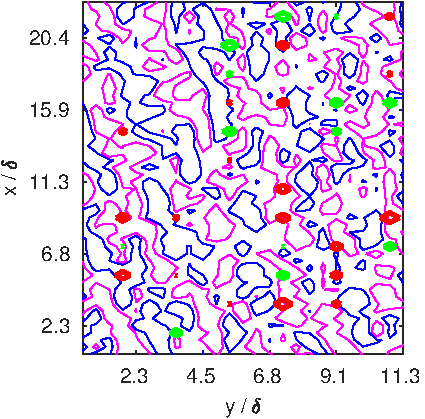
\includegraphics[width=2in,height=2in]{ek02_pi_2d_n_9_m_7_lvl_25-eps-converted-to}}}{}% 
%		  \put(0,150){(f)}
%		\end{picture}
%  \end{minipage}	  
%}
%\caption{Contour of extreme events of energy transfer between scales overlaid on u-velocity contour plots, $EK10$ case (a, b, c) and $EK02$ case (d, e, f). High velocity contours are plotted in Blue with a value of $\left < u \right >+0.5 \sigma_u$, low velocity contours are plotted in Purple with a value of $\left < u \right >-0.5 \sigma_u$. Green and Red contours are plotted for extreme events of inter-scale energy transfer between two scales for values of $-3\sigma_{t^{(m,n)}}$ and $3\sigma_{t^{(m,n)}}$, respectively. (a), (b), (c) represents energy transfer from scale $0.178\delta$, $0.348\delta$, $0.697\delta$ to a scale of spatial extent $0.178\delta$ for $EK10$ at a height of $0.515\delta$. (d), (e), (f) represents energy transfer from scale $0.454\delta$, $0.908\delta$, $1.815\delta$ to scale $0.454\delta$ for $EK02$ on a wall-parallel plane at a height of $0.49\delta$, respectively.} 
%\label{fig:inter_scale_energy_2d}
%\end{figure}

\section{Summary and Conclusions}
The existence of VLSMs as slender and elongated low- or high-momentum regions clearly marked with borders has been confirmed from visual inspection of the flow fields in the atmospheric boundary layer \citep{traumner_blm_2015}. The importance of these structures is of interest because of the fact that any turbulent flow exhibits a hierarchy of motions of different scales. The role of VLSMs in this hierarchy is not completely defined. One important aspect of VLSMs is that they influence or modulate small-scale motions and the characterization of this modulation was explored in Sec. \ref{Modulation_VLSMs}. For this analysis on modulation effect, the large scale has been defined as any motion with a scale larger than $2\delta$. The same analysis was carried out with a cut-off scale of $5\delta$ to separate large and small scales. Irrespective of the definition of large scales, qualitatively, results did not change. It was observed that large-scale fluctuations correlate with small-scale fluctuations in agreement with previous work \citep{ganapathi_jfm_2012_modulation} and that the degree of fluctuation in large scales dictates the degree of fluctuation in small scales with large fluctuations in large scales corresponding to large fluctuations in small scales. The frequency of fluctuations of small scales, however, is not strongly correlated to the strength of fluctuations of large scale in the log and outer region and appears to be a function of height. The magnitude of Reynold's stress is inversely correlated to the intensity of large-scale fluctuations. This observation bears importance in automated detection algorithms of VLSMs in any flow field and suggests that VLSMs are most likely to be found as areas characterized by lower Reynold's stresses.  

The mechanism of exerting influence on small-scale dynamics by large scales is explored through interscale energy exchange in the wavelet domain. The main question was whether nonlocal energy transfer would be responsible for the influence of VLSMs on small-scale motions. It was observed that the magnitude of nonlocal energy transfer in the three examined cases was insignificant compared to the local energy transfer. There was no evidence found that VLSM or LSM could significantly impact small-scale turbulent motions through nonlocal energy transfer. Another question was whether weak rotation would impact energy transfer between scales and ultimately impact the organization of VLSMs and LSMS. This was particularly important due to the fact that in the environment at large scales, Coriolis force cannot be ignored. Prior work has shown that for very low Rossby number including the limiting case of solid body rotation (zero $Ro$ number), the energy transfer characteristics change even though the Coriolis force is absent from the $tke$ transport equation \citep{yeung_zhou_pof_98, hossain_pof_94}. Weak rotation as has been interrogated in this study also shows its impact on the energy distribution over length scales. This is evident from the one-dimensional spectra of the streamwise velocity (Fig. \ref{fig:spectra_fw}). Unlike pressure-driven channel flow, a very narrow band of scales contain most of the $tke$ when there is a Coriolis force. This could indicate the inhibition of the development of VLSMs or shortening of the length scale of VLSMs. However, significant changes in the local, nonlocal energy transfer characteristics were not observed, an indication that the fundamental turbulent dynamics were not altered although the ratio of the largest to smallest energy containing length scales did change when Coriolis force was introduced.

As the method responsible for the organisation of VLSMs, GH12 associated the well-known paradigm of the train of hairpin vortices where counter rotating vortices align themselves along the streamwise direction spaced by the inclined, induced long regions of low- and high-speed fluids. From kinematic consideration, this scenario stands out as a possible organization of the constituent coherent structures that shape VLSMs. By coherent structures, we refer to a conglomeration of phase-correlated vortices following the definition adopted by Hussain  \citep{hussain_1983_csreality} and prefer to maintain a clear distinction between coherent structures and VLSMs,  which are often mixed up and used interchangeably in the literature. This distinction is important to maintain to understand the physical energy cascade process. Although scale-scale interaction or the turbulent energy content over scales is analysed in spectral space or wavelet space, the physical mechanism of transfer is most often explained by vorticity dynamics. There is an apparent disconnect between energy density over assumed wavelike motions, which do not really exist in a turbulent flow field, and the physical mechanism of vortex stretching or merging through which energy transfers to smaller scales or travels towards larger scales, respectively. 

The physical mechanism of energy transfer from large to smaller scales corresponds to breaking up of large energy containing coherent motions \citep[chap. 5]{davidson_turb_book}. Irrespective of the background mechanism responsible for the formation of LSMs and VLMSs, the interscale energy transfer characteristics as explored here indicate that it is possible for smaller scale motions to merge together to form large-scale motions. This prediction can be attributed to the observed transfer of energy from small to large scales. However, a hierarchy of this merging process is also observed. In general, smaller scale motions combine to form a larger scale motions and those larger scale motions would combine to form even larger scale motions. However, the reverse cascading of energy does not break the observance of Richardson's prescribed forward energy cascading. The energy transfer from large to small scales always dwarfs the energy transfer from small to large scales. The observed energy exchange process and spectra here lend support toward the hypothesis that LSMs concatenate to form VLSMs as suggested by \citet{kim_adrian_pof99, balakumar_adrian_ptrs_07, baltzer_jfm_13}.

\bibliographystyle{unsrtnat}
\bibliography{MyThesisRefs}
\clearpage
%% ======================= ALL TABLES ====================

\begin{table}
\centering
\footnotesize
\caption{Simulation parameters}
\centering
\begin{tabular}{ c c c c c c c c c c c c}
\hline 
 & Nx & Ny & Nz & $L_x$(Km) & $L_y$(Km) & $L_z$ (Km) & $U_g$ (m/s) & $u_*$ (m/s) & $\delta$(m) & $Ro$ & $f(s^{-1})$ \\
\hline 
$EK10$ & 2048 & 2048 & 64 & 120 & 120 & 1.5 & 10  & 0.41 & 1433.00  & 67 & 10$^{-4}$  \\
$EK02$ & 2048 & 2048 & 64 & 120 & 120 & 0.75 & 2 & 0.09 & 550.69 & 33 & 10$^{-4}$ \\
$CHNL$ & 2048 & 2048 & 64 & 120 & 120 & 1.5 & 0 & 0.42  & 1500.00 & - & - \\
\hline 
\hline 
\end{tabular}
\label{tab:sim_param}
\end{table}

\begin{table}
	  \caption{Wavelet decomposition levels and corresponding normalised horizontal length scales ($r_m/\delta$) and wavenumbers ($k_m\delta$) of all three cases.}	
	    \centering
		\begin{tabular}{cllllllll}
		\hline \hline\\
		Wavelet Decomposition Level (m/n) &  \multicolumn{2}{c}{CHNL} &  & \multicolumn{2}{c}{EK10} & & \multicolumn{2}{c}{EK02}\\
		\hline \\
		{}   & {$r_{m}/\delta$}   & {$k_m\delta$}  &   & {$r_{m}/\delta$}    & {$k_{m}\delta$} &  & {$r_{m}/\delta$}   & {$k_{m}\delta$} \\
		1  & 42.666 & 0.147   &   &  44.66    & 0.140  &  & 116.21    & 0.0541 \\ 
		2  & 21.333 & 0.294   &   &  22.33    & 0.281  &  & 58.109    & 0.1081 \\
		3  & 10.666 & 0.589   &   &  11.16    & 0.562  &  & 29.054    & 0.2163 \\
		4  & 5.333  & 1.178   &   &  5.582    & 1.125  &  & 14.527    & 0.4325 \\
		5  & 2.666  & 2.356   &   &  2.791    & 2.250  &  & 7.2637    & 0.8650 \\
		6  & 1.333  & 4.712   &   &  1.395    & 4.501  &  & 3.6319    & 1.7300 \\
		7  & 0.666  & 9.424   &   &  0.697    & 9.003  &  & 1.8159    & 3.4600 \\
		8  & 0.33   & 18.849  &   &  0.348    & 18.00  &  & 0.9080    & 6.9201 \\
		9  & 0.166  & 37.699  &   &  0.174    & 36.01  &  & 0.4540    & 13.840 \\
		10 & 0.083  & 75.398  &   &  0.087    & 72.02  &  & 0.2270    & 27.680 \\
		\hline\hline
		\end{tabular}	
	
	\label{tab:wav-mode2scale}
\end{table}
% ================ ALL FIGURES =============================
% ------------------- modulation ------------------------
\graphicspath{{chap2Img/}}
\begin{figure}[htb]
\centering {
	\begin{minipage}{0.99\textwidth}
	\setlength{\unitlength}{1in}
	  \begin{picture}(6.5,5.5)
		  \put(0,0){{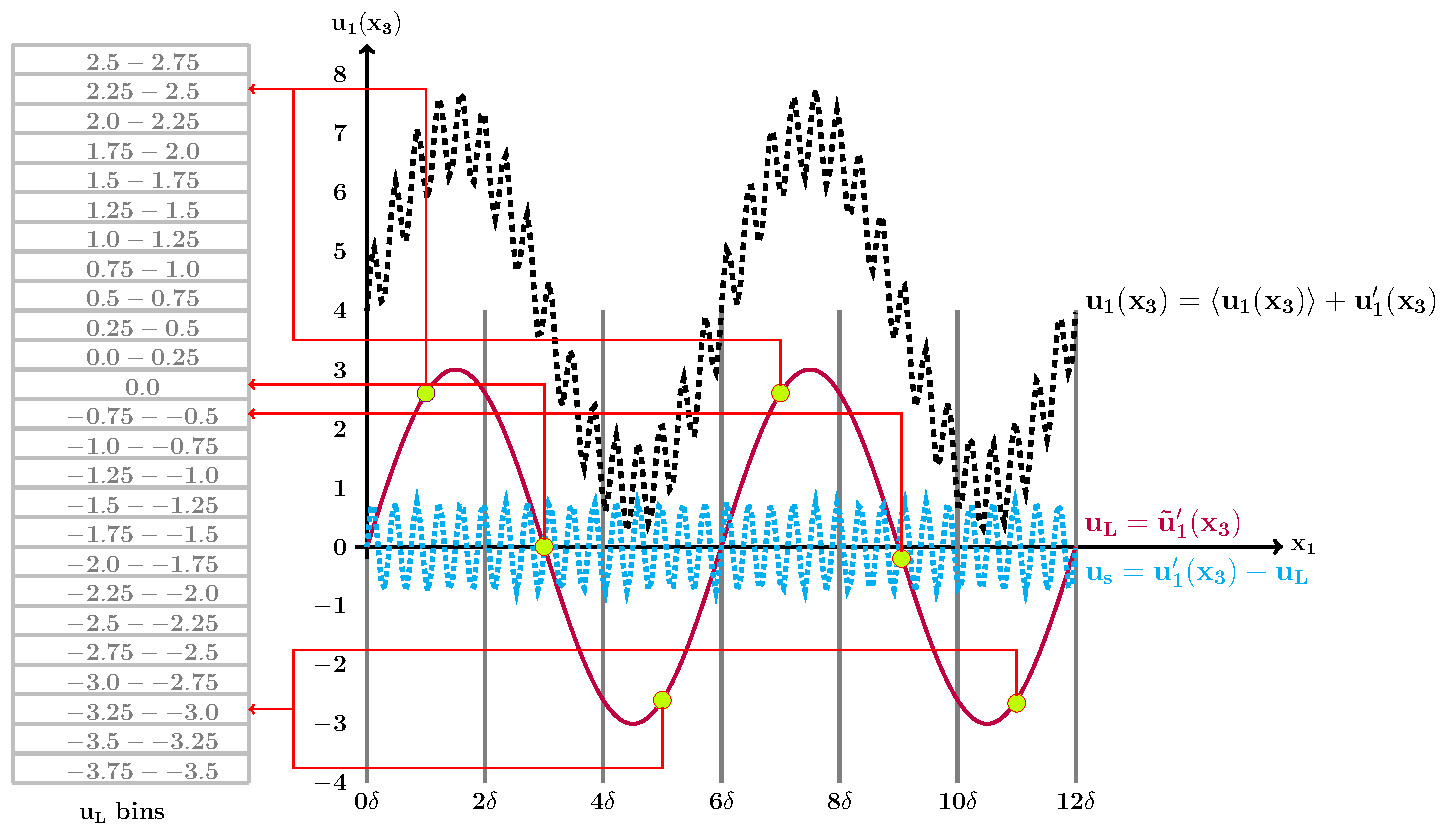
\includegraphics[width=6.0in,height=5.5in]{modulation_diagram}}}{}% 
		\end{picture}
	\end{minipage}%
	}
\caption{An illustration of the data extraction method used to investigate the modulation of the small-scale motions by large-scale motions is shown. The black dashed line in the figure represents a raw velocity signal ($u_1(x_3)$) extracted along a line in $x_1$-direction from the simulated flow field. The filtered large-scale fluctuation ($u_L$) is represented by the red smooth line. The dotted blue line represents the data series of small-scale fluctuation ($u_s$). On the left, a hypothetical binning process for the $u_L$ series is shown and  the association of the representative $u_L$ values to the correct bin is shown with arrows.}
\label{fig:modulation}
\end{figure}

% ============== variation of us2 as a function of z for different uL ======================
\graphicspath{{chap2Img/}}
\begin{figure}[htb]
\centering {
	\begin{minipage}{0.333\textwidth}
	  \begin{picture}(100,150)
		  \put(-5,0){{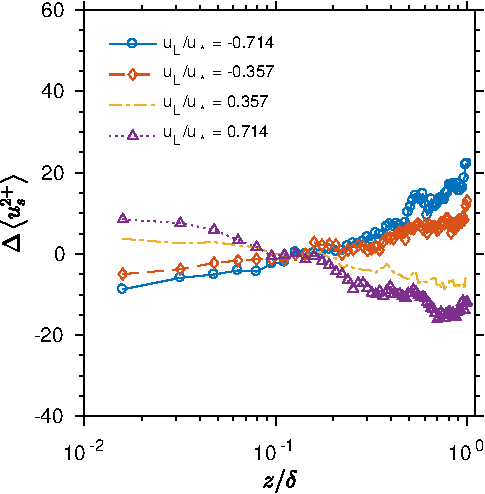
\includegraphics[width=2in,height=2in]{chnl_u_s2_z_multiple_u_l_0-eps-converted-to}}}{}% 
		  \put(40,30){(a)}
		\end{picture}
	\end{minipage}%
	\begin{minipage}{0.3333\textwidth}
	    \begin{picture}(100,150)
		    \put(0,0){{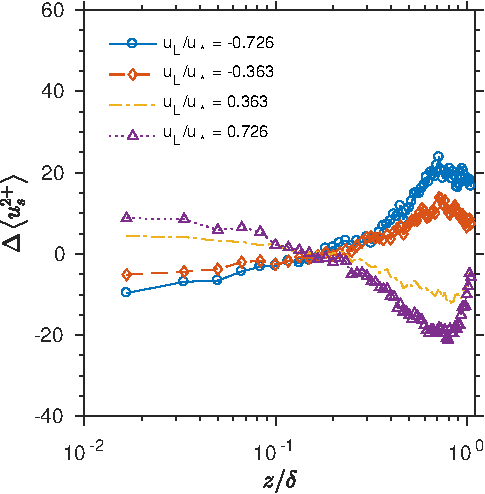
\includegraphics[width=2in,height=2in]{ek10_u_s2_z_multiple_u_l_0-eps-converted-to}}}{}% 
		    \put(40,30){(b)}
		  \end{picture}
	\end{minipage}%	
	\begin{minipage}{0.34\textwidth}
	  \begin{picture}(100,150)
		  \put(0,0){{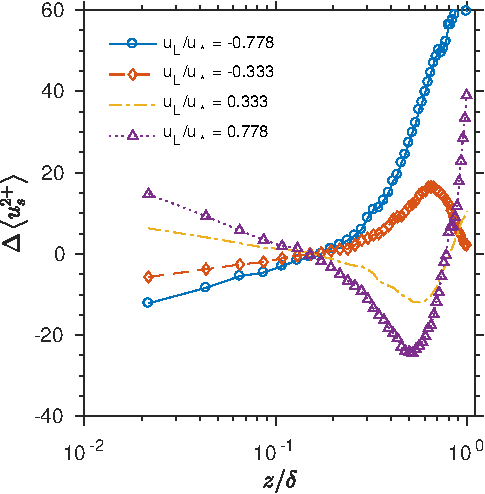
\includegraphics[width=2in,height=2in]{ek02_u_s2_z_multiple_u_l_0-eps-converted-to}}}{}% 
		  \put(40,30){(c)}
		\end{picture}
  \end{minipage}	    
}
\caption{The relative strength of small-scale fluctuations conditioned on the strength of fluctuations of large scales as defined in Eq. \ref{eq:relative_var_us2} for the three different flow cases, (a) $CHNL$, (b) $EK10$, and (c) $EK02$.}
\label{fig:us2_uL}
\end{figure}

% =============== variation of kx_us as a function of z for different uL ======================
\graphicspath{{chap2Img/}}
\begin{figure}[htb]
\centering {
	\begin{minipage}{0.333\textwidth}
	  \begin{picture}(100,150)
		  \put(0,0){{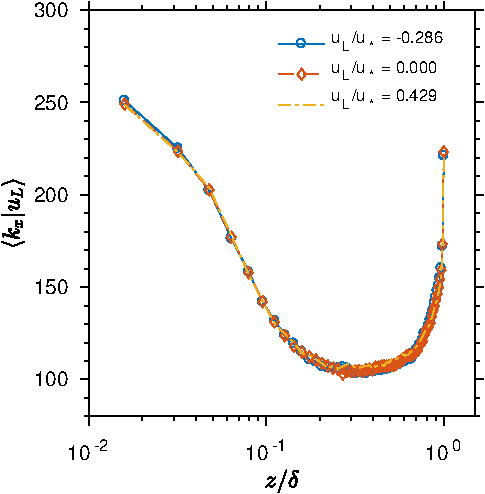
\includegraphics[width=2in,height=2in]{chnl_kx_ul_z-eps-converted-to}}}{}% 
		  \put(35,30){(a)}
		\end{picture}
	\end{minipage}%
	\begin{minipage}{0.333\textwidth}
	    \begin{picture}(100,150)
		    \put(0,0){{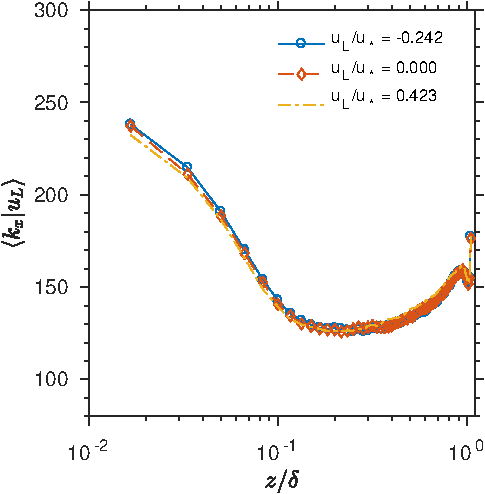
\includegraphics[width=2in,height=2in]{ek10_kx_ul_z-eps-converted-to}}}{}% 
		    \put(35,30){(b)}
		  \end{picture}
	\end{minipage}%	
	\begin{minipage}{0.334\textwidth}
	  \begin{picture}(100,150)
		  \put(0,0){{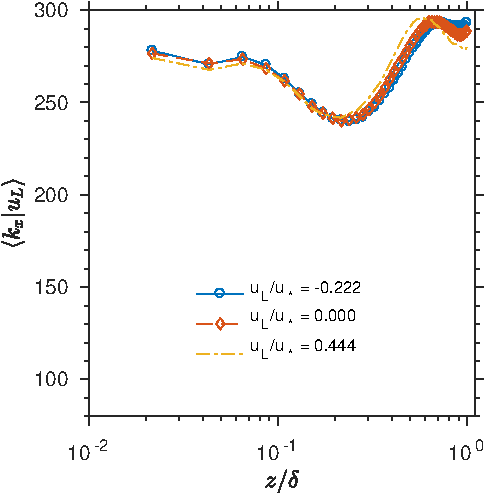
\includegraphics[width=2in,height=2in]{ek02_kx_ul_z-eps-converted-to}}}{}% 
		  \put(35,30){(c)}
		\end{picture}
  \end{minipage}	
}
\caption{The wavenumber quantifying the scale of fluctuation of primary turbulent motions as a function of large-scale fluctuation intensities for the three cases, (a) $CHNL$, (b) $EK10$, and (c) $EK02$.}
\label{fig:kx_ul}
\end{figure} 


% ===== variation of u'w' as a function of z for different uL ======================
\graphicspath{{chap2Img/}}
\begin{figure}[htb]
\centering {
	\begin{minipage}{0.333\textwidth}
	  \begin{picture}(100,150)
		  \put(0,0){{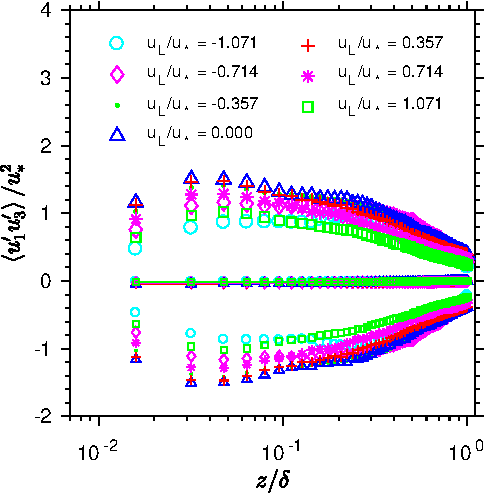
\includegraphics[width=2in,height=2in]{chnl_u_l_uw_std-eps-converted-to}}}{}% 
		  \put(28,30){(a)}
		\end{picture}
	\end{minipage}%
	\begin{minipage}{0.333\textwidth}
	    \begin{picture}(100,150)
		    \put(0,0){{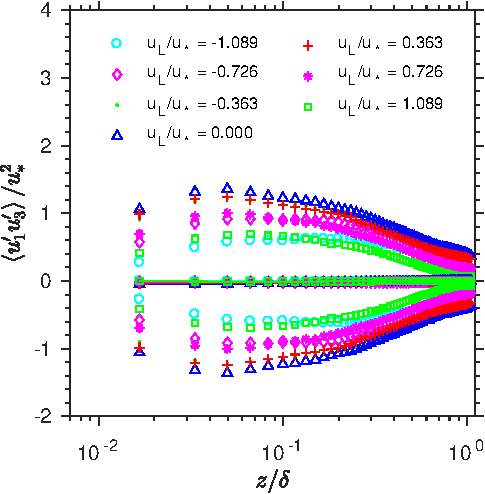
\includegraphics[width=2in,height=2in]{ek10_u_l_uw_std-eps-converted-to}}}{}% 
		    \put(28,30){(b)}
		  \end{picture}
	\end{minipage}%	
	\begin{minipage}{0.334\textwidth}
	  \begin{picture}(100,150)
		  \put(0,0){{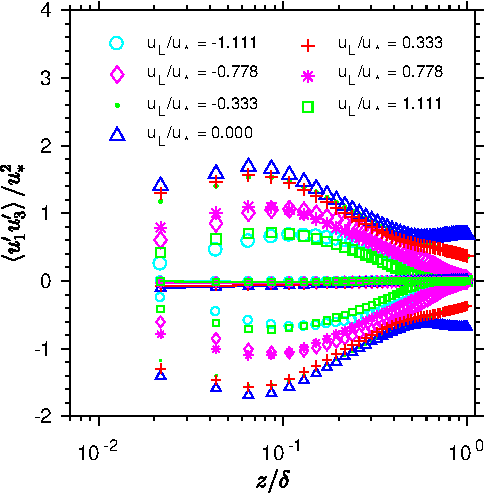
\includegraphics[width=2in,height=2in]{ek02_u_l_uw_std-eps-converted-to}}}{}% 
		  \put(28,30){(c)}
		\end{picture}
  \end{minipage}	
}
\caption{The wall-normal Reynolds shear stress, $u^\prime w^\prime$, normalized by the surface shear stress as a function of large-scale fluctuations and distance in the wall-normal direction for each of the cases, (a) $CHNL$, (b) $EK10$, and (c) $EK02$. Solid lines correspond to the mean shear stress, $\left< u^\prime w^\prime \right>_{u_L}$, and points correspond to $\pm 3 \sigma_{u_L}^{u^\prime w^\prime}$.} 
\label{fig:uw_uL}
\end{figure}

%========================== Figure: Spectra ====================================
\graphicspath{{chap2Img/}}
\begin{figure}[htb]
\centering {
	\begin{minipage}{0.33\textwidth}
	\setlength{\unitlength}{1in}
	\begin{picture}(2.1,2)
		\put(0,0){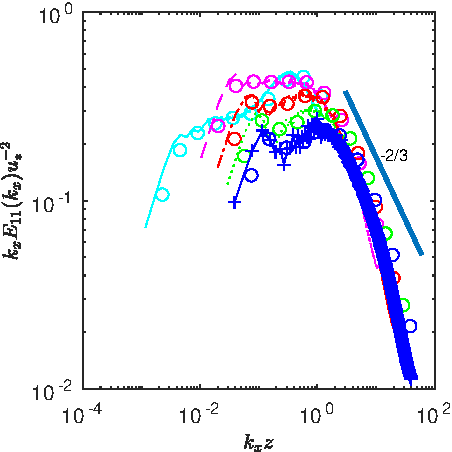
\includegraphics[width=1.9in,height=2in]{wavelet_n_fourier_spectra_chnl_pre-eps-converted-to}}{}% 
		\put(0.45,0.45){($\mathbf{a}$)}
	\end{picture}	
	\end{minipage}%
	\begin{minipage}{0.33\textwidth}
	\setlength{\unitlength}{1in}
	\begin{picture}(2.1,2)
		\put(0,0){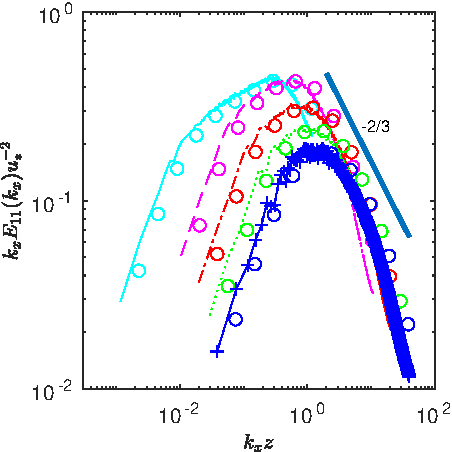
\includegraphics[width=1.9in,height=2in]{wavelet_n_fourier_spectra_ek10_pre-eps-converted-to}}{}%
		\put(0.45,0.45){($\mathbf{b}$)}
		\end{picture}
	\end{minipage}%	
		\begin{minipage}{0.33\textwidth}
		\setlength{\unitlength}{1in}
		\begin{picture}(2.1,2)
	  \put(0,0){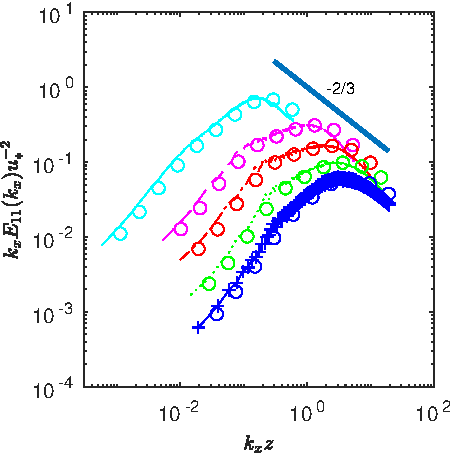
\includegraphics[width=1.9in,height=2in]{wavelet_n_fourier_spectra_ek02_pre-eps-converted-to}}{}%
	  \put(0.45,0.45){($\mathbf{c}$)}
	  \end{picture}
\end{minipage}	
}
\caption{Premultiplied wavelet and Fourier spectra of streamwise velocity component, averaged over spanwise direction for (a) $CHNL$, (b) $EK10$, and (c) $EK02$ at different wall-normal locations. Spectra are plotted against wavenumbers normalized by height. Lines represent Fourier spectra and circles represent wavelet spectra. Line types {\tiny ---,$--$, $- \cdot$, $\cdot \cdot \cdot$, $-+$}  correspond to heights ($0.01\delta$, $0.14\delta$, $0.26\delta$, $0.39\delta$, $0.52\delta$) for $CHNL$, ($0.01\delta$, $0.14\delta$, $0.28\delta$,$0.41\delta$, $0.54\delta$) for $EK10$, and ($0.04\delta$, $0.19\delta$, $0.34\delta$, $0.54\delta$, $0.71\delta$) for $EK02$.}
\label{fig:spectra_fw}
\end{figure}

\graphicspath{{chap2Img/}}
\begin{figure}[htb]
	\begin{minipage}{\textwidth}
	\setlength{\unitlength}{1in}
	  \begin{picture}(6,4)
		\put(0.5,0){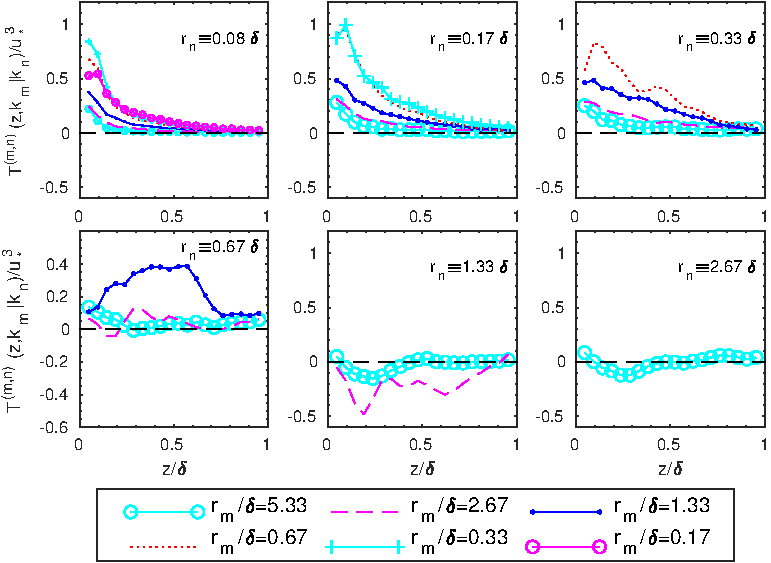
\includegraphics[width=5.0in,height=3.9in]{tmn_chnl_fixed_n-eps-converted-to}}
	%	\put(-0.1,2.5){$\mathbf{(a)}$}
	  \end{picture}
	\end{minipage}
\caption{Wavelet dual bi-spectrum of subgrid scale transfer normalized by $u_*^3$ for the $CHNL$ case. This figure shows the rate of energy transfer over unit area per unit length of scale where energy transfer occurs from scales $r_{m}/\delta$ to scales smaller than $r_{n}/\delta$.}	
\label{fig:tmn_fixed_n_chnl}
\end{figure}%
\begin{figure}
	\begin{minipage}{\textwidth}
	\setlength{\unitlength}{1in}
	\begin{picture}(6,4)
		\put(0.5,0){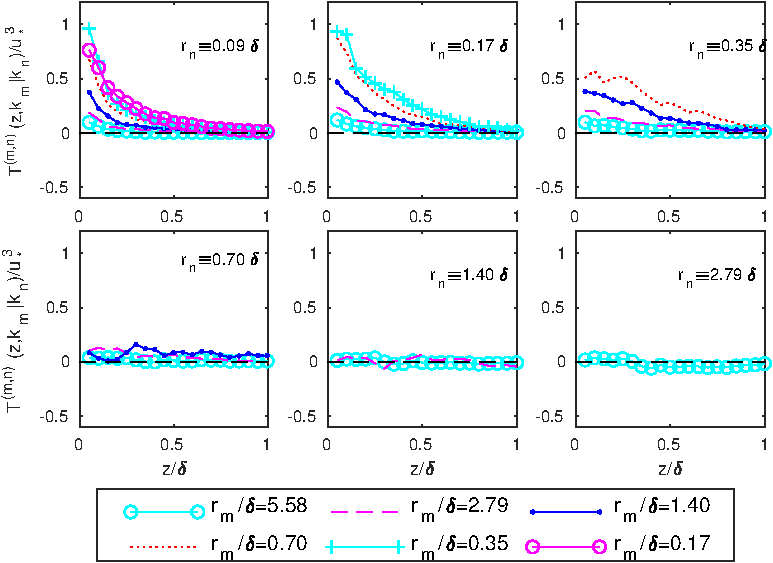
\includegraphics[width=5.0in,height=3.9in]{tmn_ek10_fixed_n-eps-converted-to}}
		%\put(-0.1,2.5){$\mathbf{(b)}$}
	\end{picture}
	\end{minipage}
\caption{The rate of energy transfer over unit area per unit length of scale is shown for the $EK10$ case where energy transfer occurs from scales $r_{m}/\delta$ to scales smaller than $r_{n}/\delta$. Energy transfer is normalized by $u_*^3$. }	
\label{fig:tmn_fixed_n_ek10}
\end{figure}

\begin{figure}	
	\begin{minipage}{\textwidth}
	\setlength{\unitlength}{1in}
	\begin{picture}(6,4)
	\put(0.5,0){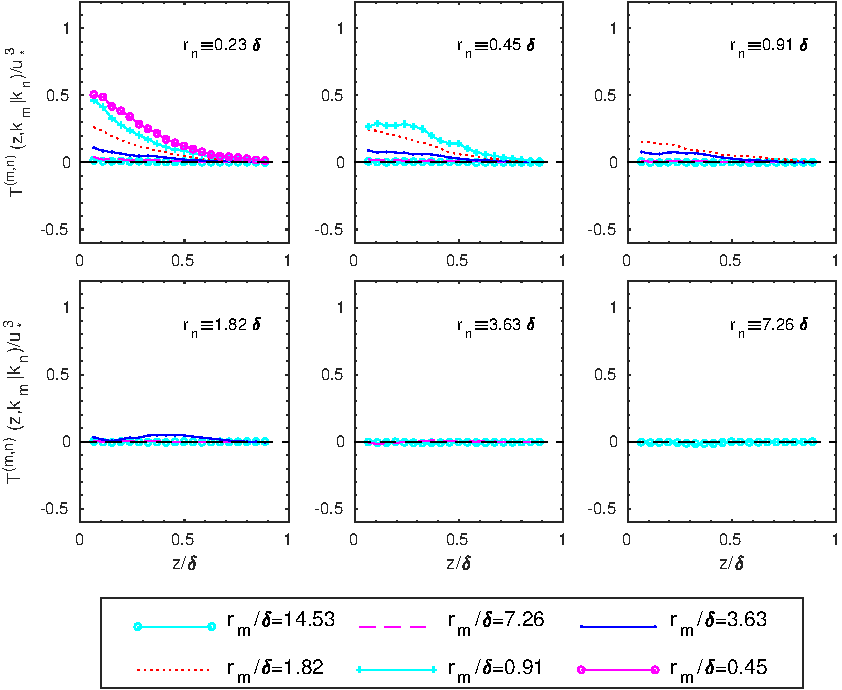
\includegraphics[width=5.0in,height=3.9in]{tmn_ek02_fixed_n-eps-converted-to}}
	%\put(-0.1,2.5){$\mathbf{(c)}$}
	\end{picture}
\end{minipage}	
\caption{Wavelet dual bi-spectrum of subgrid scale transfer normalised by $u_*^3$ for $EK02$. Energy transfer is measured over unit area per unit length of scale and transfer occurs from scales $r_{m}/\delta$ to scales smaller than $r_{n}/\delta$.}
\label{fig:tmn_fixed_n_ek02}
\end{figure}%


\graphicspath{{chap2Img/}}
\begin{figure}
	\begin{minipage}{\textwidth}
	\setlength{\unitlength}{1in}
	  \begin{picture}(6,4)
		\put(0.5,0){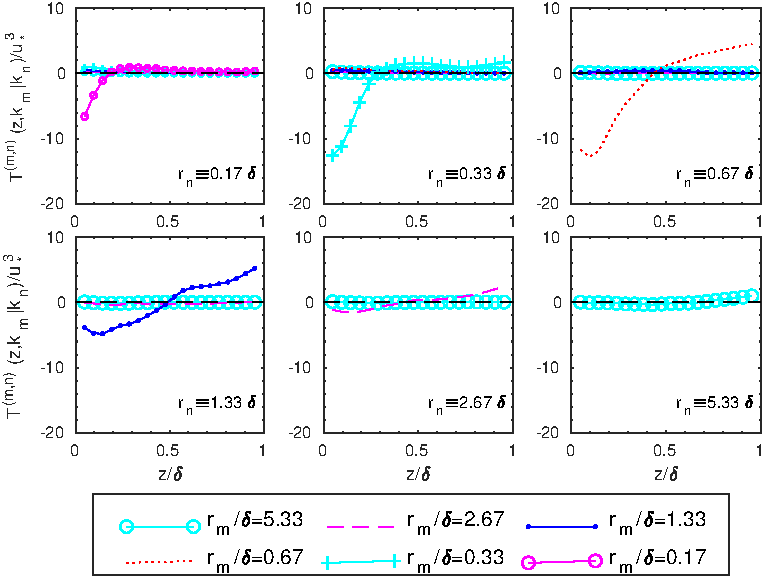
\includegraphics[width=5.0in,height=3.9in]{tmn_chnl_fixed_n-m_n_equal-eps-converted-to}}
		%\put(-0.1,2.5){$\mathbf{(a)}$}
	  \end{picture}
	\end{minipage}
\caption{Wavelet dual bi-spectrum of subgrid scale transfer normalised by $u_*^3$ for the $CHNL$ case. In contrast to Fig. \ref{fig:tmn_fixed_n_chnl}, this figure shows the transfer occurring between length scales $r_m$ to $r_m$ ($r_n \equiv r_m$)}	
\label{fig:tmn_fixed_n_meqn_chnl}
\end{figure}

\begin{figure}
	\begin{minipage}{\textwidth}
	\setlength{\unitlength}{1in}
	\begin{picture}(6,4)
		\put(0.5,0){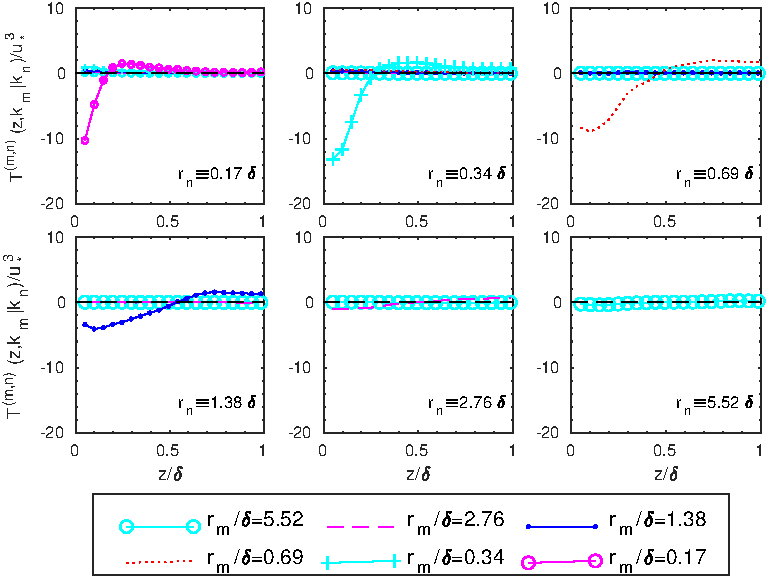
\includegraphics[width=5.0in,height=3.9in]{tmn_ek10_fixed_n-m_n_equal-eps-converted-to}}
		%\put(-0.1,2.5){$\mathbf{(b)}$}
	\end{picture}
	\end{minipage}
\caption{Wavelet dual bi-spectrum of subgrid scale transfer normalised by $u_*^3$ for the $EK10$ case. In contrast to Fig. \ref{fig:tmn_fixed_n_ek10}, this figure shows the transfer occurring between length scales $r_m$ to $r_m$ ($r_n \equiv r_m$)}	
\label{fig:tmn_fixed_n_meqn_ek10}
\end{figure}
	
\begin{figure}
	\begin{minipage}{\textwidth}
	\setlength{\unitlength}{1in}
	\begin{picture}(6,4)
	\put(0.5,0){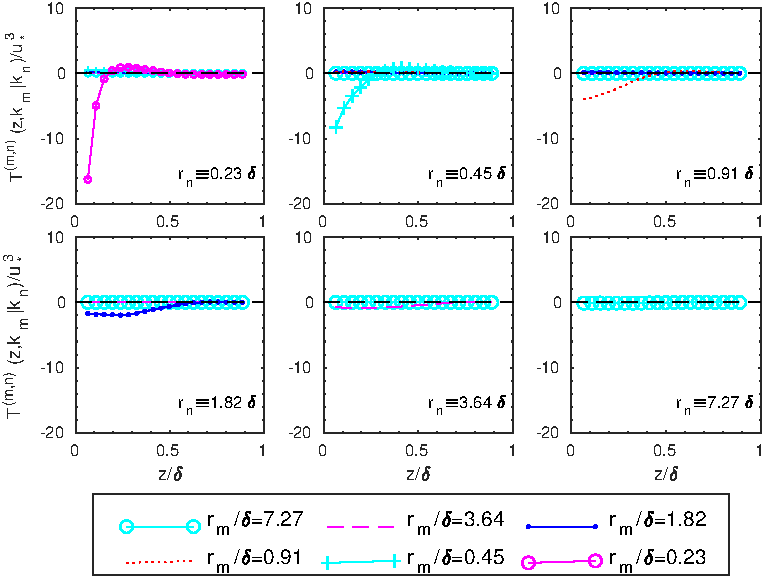
\includegraphics[width=5.0in,height=3.9in]{tmn_ek02_fixed_n-m_n_equal-eps-converted-to}}
	%\put(-0.1,2.5){$\mathbf{(c)}$}
	\end{picture}
\end{minipage}	
\caption{Wavelet dual bi-spectrum of subgrid scale transfer normalised by $u_*^3$ for the $EK02$ case. The energy transfer from scale $r_m$ to $r_n (\equiv r_m)$ is shown in contrast to Fig. \ref{fig:tmn_fixed_n_ek02} where, $r_n < \frac{1}{2}r_m$.}
\label{fig:tmn_fixed_n_meqn_ek02}
\end{figure}%

\graphicspath{{chap2Img/}}
\begin{figure}
\centering {
	\begin{minipage}{0.5\textwidth}
	  \begin{picture}(100,180)
		  \put(0,-5){{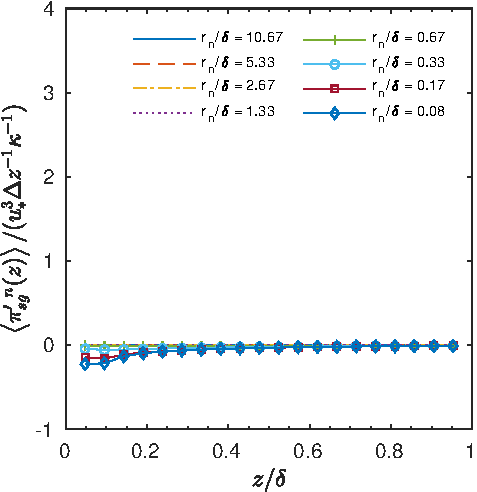
\includegraphics[width=2.85in,height=2.37in]{pi_chnl_diff_n_by_u3_dz_2-eps-converted-to}}}
		  \put(0,150){($a$)}
		\end{picture}
	\end{minipage}%
	\begin{minipage}{0.49\textwidth}
	    \begin{picture}(100,180)
		    \put(0,-5){{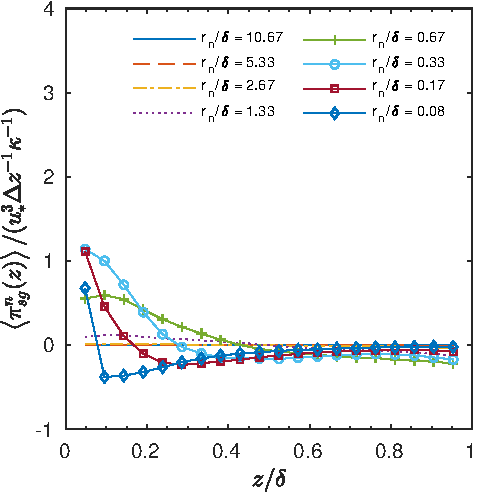
\includegraphics[width=2.85in,height=2.37in]{pi_chnl_diff_n_by_u3_dz-eps-converted-to}}}
		    \put(0,150){($a^\prime$)}
		  \end{picture}
	\end{minipage}%
		
	\begin{minipage}{0.5\textwidth}
	  \begin{picture}(100,180)
		  \put(0,-5){{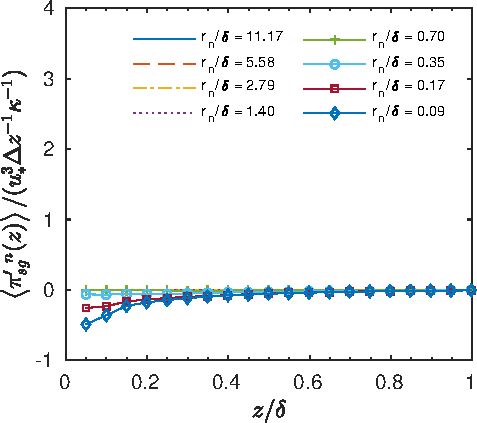
\includegraphics[width=2.85in,height=2.37in]{pi_ek10_diff_n_by_u3_dz_2-eps-converted-to}}} 
		  \put(0,150){($b$)}
		\end{picture}
  \end{minipage}	
	\begin{minipage}{0.49\textwidth}
  \begin{picture}(100,180)
	  \put(0,-5){{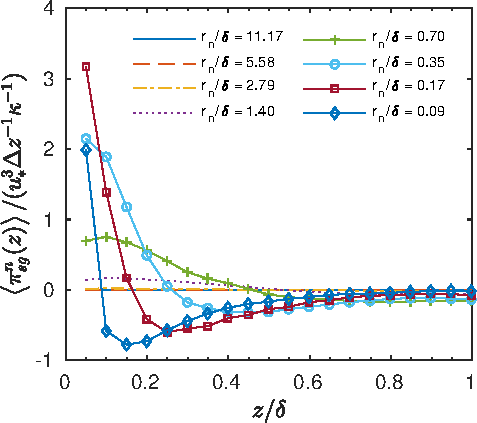
\includegraphics[width=2.85in,height=2.37in]{pi_ek10_diff_n_by_u3_dz-eps-converted-to}}}
	  \put(0,150){($b^\prime$)}
	\end{picture}
  \end{minipage}

	\begin{minipage}{0.5\textwidth}
	  \begin{picture}(100,180)
		  \put(0,-5){{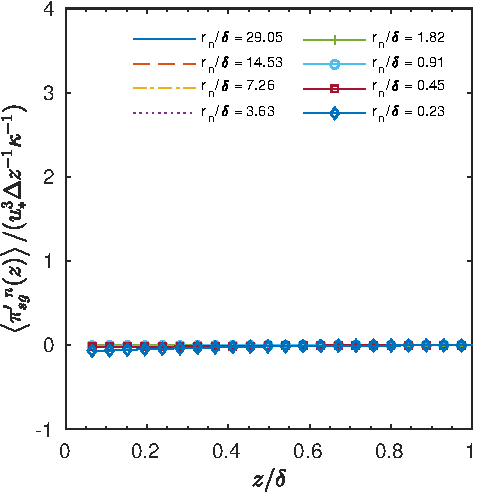
\includegraphics[width=2.85in,height=2.37in]{pi_ek02_diff_n_by_u3_dz_2-eps-converted-to}}} 
		  \put(0,150){($c$)}
		\end{picture}
  \end{minipage}	
	\begin{minipage}{0.49\textwidth}
  \begin{picture}(100,180)
	  \put(0,-4){{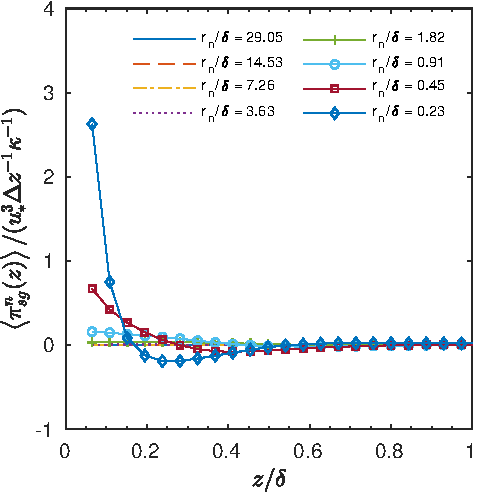
\includegraphics[width=2.85in,height=2.37in]{pi_ek02_diff_n_by_u3_dz-eps-converted-to}}} 
	  \put(0,150){($c^\prime$)}
	\end{picture}
\end{minipage}
}
\caption{Aggregate subgrid scale energy transfer from large to small scales separated by an arbitrary cut-off scale. For panels on the left, total subgrid transfer is calculated using Eqn. \ref{pi_tmn_1} and the right-hand side panels correspond to total subgrid transfer calculated following the definition in Eqn. \ref{pi_tmn}. }
\label{fig:pi_tmn}
\end{figure}
%=========================================================
